\chapter{Theory  \today}
\label{cha:theory}
\textit{by Olaf Kolditz, Norbert B�ttcher and Uwe-Jens G�rke}

Concerning the theoretical background of flow, transport, deformation, and reaction processes in porous media,
there is a considerable amount of monographic literature available \cite{Bea:72,Die:85,Ehl:89,BeaBac:90,Kin:1992,Hel:97,LewSch:98,Boe:00}.
%
The idea of this chapter is to provide a concise brief-as-possible description (compendium-like) of governing equations for thermo-hydro-mechanical / chemical [THM/C] processes in porous media. We will point to literature references rather than giving detailed derivations of the governing equations. This part is the theoretical basis for all benchmarks and examples upcoming in part II and III of this book. We will refer to this part in the examples sections where the working equations are briefly repeated. A list of symbols can be found in the Appendix.

From the mechanical point of view we consider non-isothermal flow of multiple fluid phases (compressible and incompressible fluids) in a deformable thermo-poro-elastic porous medium based on Biot's consolidation concept.
A short introduction to continuum mechanics is given in section \ref{sec:continum_mechanics},
followed by basic conservations principles (section \ref{sec:conservation_principles}) as well as an introduction to theory of porous medium (section \ref{sec:porous_medium}).
%
The followings steps are conducted to derive the general field equations:
\begin{itemize}
 \item Macroscopic balance equations for mass, momentum and energy conservation of porous media (section \ref{sec:balance_equations}),
 \item Constitutive relationships for non-isothermal multiphase flow and deformation processes in porous media, 
 (sections \ref{sec:fluid_properties} and \ref{sec:m_properties}),
 \item Applying the constitutive relationships and introducing physically based simplifications to the balance equations for the derivation of the general field equations. 
 (parts II and III).
\end{itemize}

%-------------------------------------------------------------------------
\section{Continuum mechanics}
\label{sec:continum_mechanics}
%\section{Continuum mechanics}

The basic idea of continuum mechanics is
that the evolution of a physical system is completely determined by conservation laws,
i.e. basic properties such as mass, momentum, and energy are conserved
during the considered process at all times.
Any physical system can be completely determined by these conservation properties.
In contrast,
other quantities such as pressure or entropy do not obey conservation laws.
The only additional information concerns the consistence of the material
(e.g. fluids, solids, porous medium) in form of constitutive laws.

The concept of conservation means
that the variation of a conservation quantity within a given control volume
is due to the net effect of internal {\it sources} and
of the amount of the quantity which is crossing the boundary surface
of the considered volume - {\it fluxes}.
Sources and fluxes are, in general, dependent of space-time coordinates as well as
on mechanical and thermodynamic factors.
Fluxes result from two contributions:
first due to advective transport by fluid motion and
second due to diffusion/dispersion processes.
Diffusion is always present even when the fluid is at rest.
Diffusion is the tendency towards equilibrium or homogeneity
of a physical system.

%-------------------------------------------------------------------------
%\subsection{Preliminary remarks}
%\label{sec:prelim}

The mechanical description of coupled thermo-hydro-mechanical (THM) processes in porous media is closely associated with the deformation of the solid phase, and the interaction of deformation and flow processes. Each solid material body (including the solid phase of a porous medium) can exhibit different kinds of motion (section \ref{sec:kinematics}):

\begin{itemize}
\item rigid body motion (translation or rotation of the body without changing its volume or shape), and
\item deformation (local relative change of lengths and/or angles referred to neighboring particles, resulting in variations of the shape and/or volume of the material body under consideration).
\end{itemize}

Deformation processes of a porous medium interact with hydraulic processes of the coupled physical system particularly in the following way:

\begin{itemize}
\item effects on the stress state within the solid phase due to pore pressure evolution (with possible risk of rock failure), and
\item variations of the pore size distribution due to the deformation of the solid skeleton, which affect the hydraulic properties, and thus, have an impact on the flow processes in the porous medium.
\end{itemize}

The analysis of deformation processes considered as mechanical response of the material body to the action of applied external forces is one of the objects of mechanics (micromechanics, continuum mechanics, CITATIONS). Porous media distinguish themselves by a sophisticated complex microstructure, whose realistic simulation is extremely challenging, and from a practical point of view generally not efficient. Therefore, continuum mechanics (which is based on the assumption that matter is continuously distributed in space) provides the preferred approaches for the mathematical modeling of deformation processes in porous media. Appropriate models are not based on a physical characterization of the real microstructure, but consider their effects on the physical behavior in a phenomenological manner (section \ref{sec:porous_medium}).

General statements of mechanics, which are independent of the specific material under consideration, refer to the kinematics of motion (shortly described in a following section) and the balance relations (section~\ref{sec:balance_equations}). By contrast, individual material dependent statements refer to the constitutive relations (section.~\ref{sec:m_properties}). Just both the balance relations as well as the constitutive relations constitute a mathematically closed system of equations to solve initial-boundary value problems of mechanics.

%-------------------------------------------------------------------------
%\section{Kinematics of continua}

% *** EPS-Grafik ***
\begin{figure}[htb!]
\begin{center}
\footnotesize
%\includegraphics[height=5.973cm,width=11.507cm]{../figures/figure1.bmp}
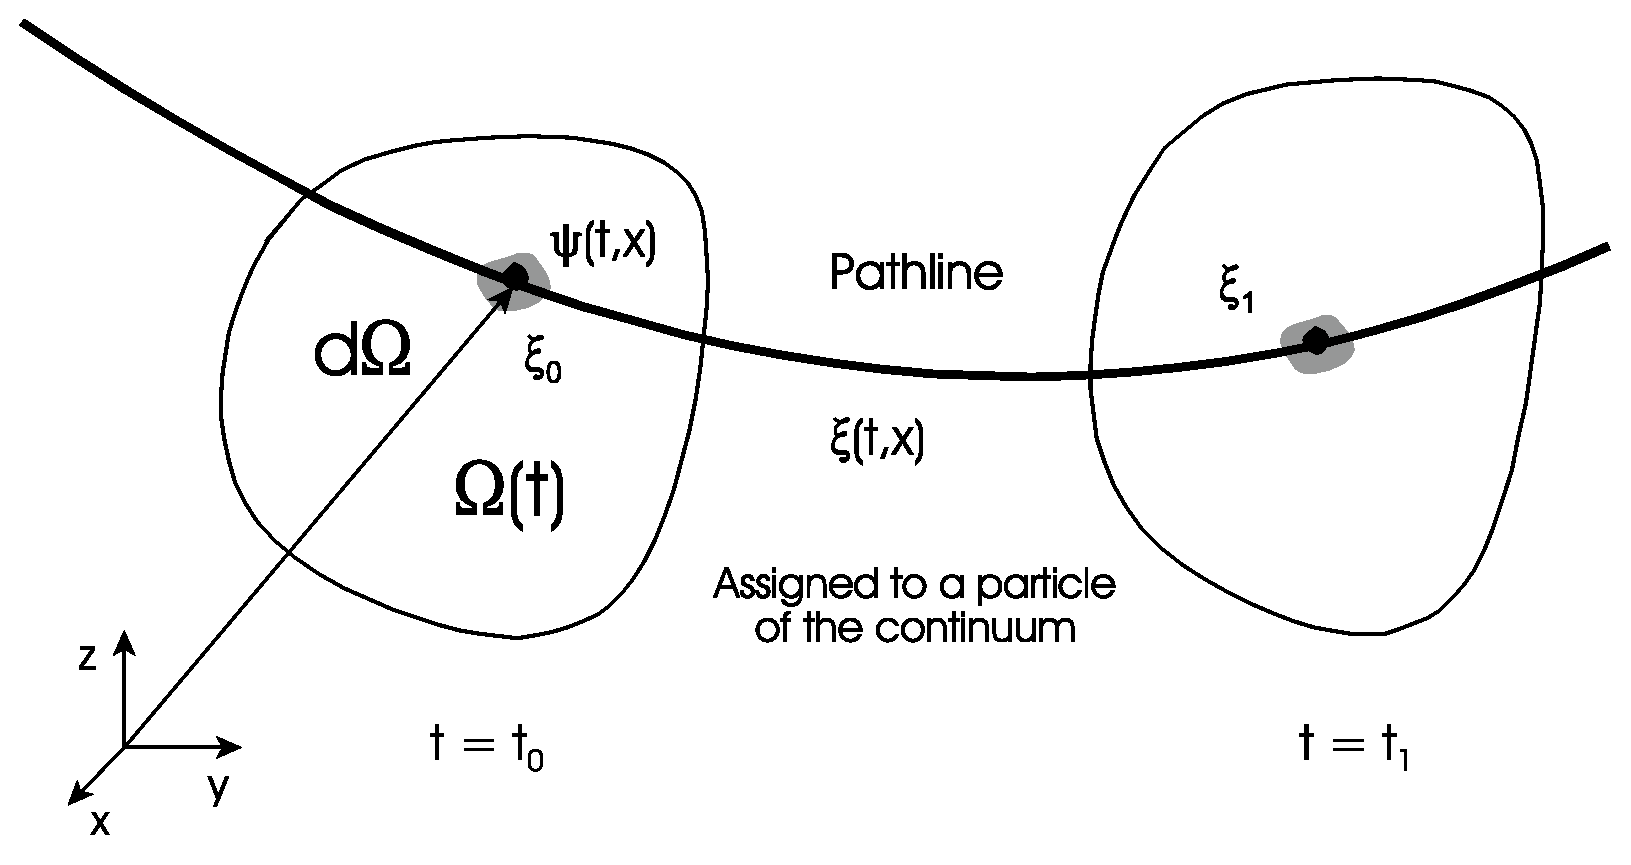
\includegraphics[width=0.8\columnwidth]{figures/mech1.eps}
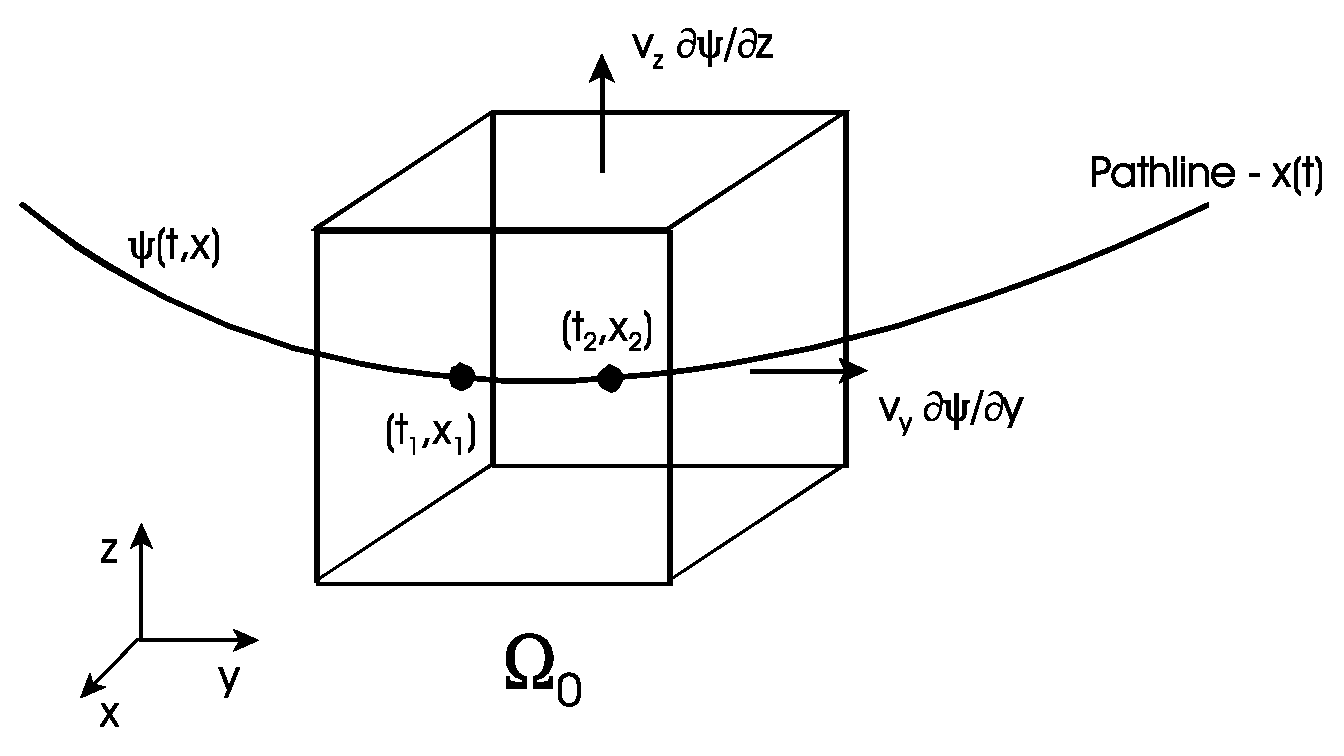
\includegraphics[width=0.8\columnwidth]{figures/mech2.eps}
\caption{Two basic descriptions of motion - Langrangian (top) and Eulerian principles (bottom), adopted from \cite{Kol:02}}
\label{fig:Euler-Langrange}
\end{center}
\end{figure}

\subsection{Lagrangian and Eulerian principles}
\label{sec:euler_lagrange}

In the {Lagrangian formulation}\index{formulation - Lagrangian} we
follow the quantity along a pathline, i.e. following particles
(Fig. \ref{fig:Euler-Langrange}, top). In the {Eulerian
formulation}\index{formulation - Eulerian} of motion we consider
variations of the quantity with respect to a fixed control
volume\index{volume - control} at fixed places (Fig.
\ref{fig:Euler-Langrange}, bottom).

A {pathline}\index{flow - pathline} is a curve along which a fixed
particle of a continuum moves during a sequence of time. Pathline
is Lagrangian concept of motion. A
{streamline}\index{flow - streamline} is a curve along which a
sequence of particles moves at a given time. By definition, the
tangent to a streamline coincides with the velocity vector at that
point. Streamline is Eulerian concept of motion. Note, for
unsteady flow the streamline may vary from one instant to the
next, whereas for steady flow streamlines remain unchanged with
time. For steady motion both pathlines and streamlines coincide.
Any particle will remain on a given streamline as time proceeds.
Additional terms associated with kinematics of continua are the
following (see also section \ref{sec:kinematics}).

\subsection{Kinematics of continua}
\label{sec:kinematics}

Kinematics analyzes the geometry of motion in general, and of deformation processes in particular. It is based on the assumption that a material (physical) body $\mathcal{B}$, which represents a set of elements $\mathcal{P}$ called material points (aka: material elements, particles), at each moment of time can be uniquely defined with certain parts (usually different if motion occurs) of space. Assigning the material body particularly to its image in the three-dimensional Euclidean space of physical observations, the location of each material point at each time can be identified with the position vector $\mathbf{x}(t)$ in a physically well-founded manner. Consequently, the position vector can be represented by its Cartesian coordinates $x_1,\,x_2,\,x_3$. In order to characterize the motion of a material body uniquely with respect to a reference state, the domain in space occupied by the material body at an arbitrarily selected time $t_0$ is of an emphasized significance. Usually in porous media mechanics, an appropriately chosen initial state of the solid skeleton is chosen as the reference state. The position vectors to define the positions of the material points at $t_0$ are denoted as $\mathbf{X}$.

\begin{figure}[htb!]
\begin{center}
\footnotesize
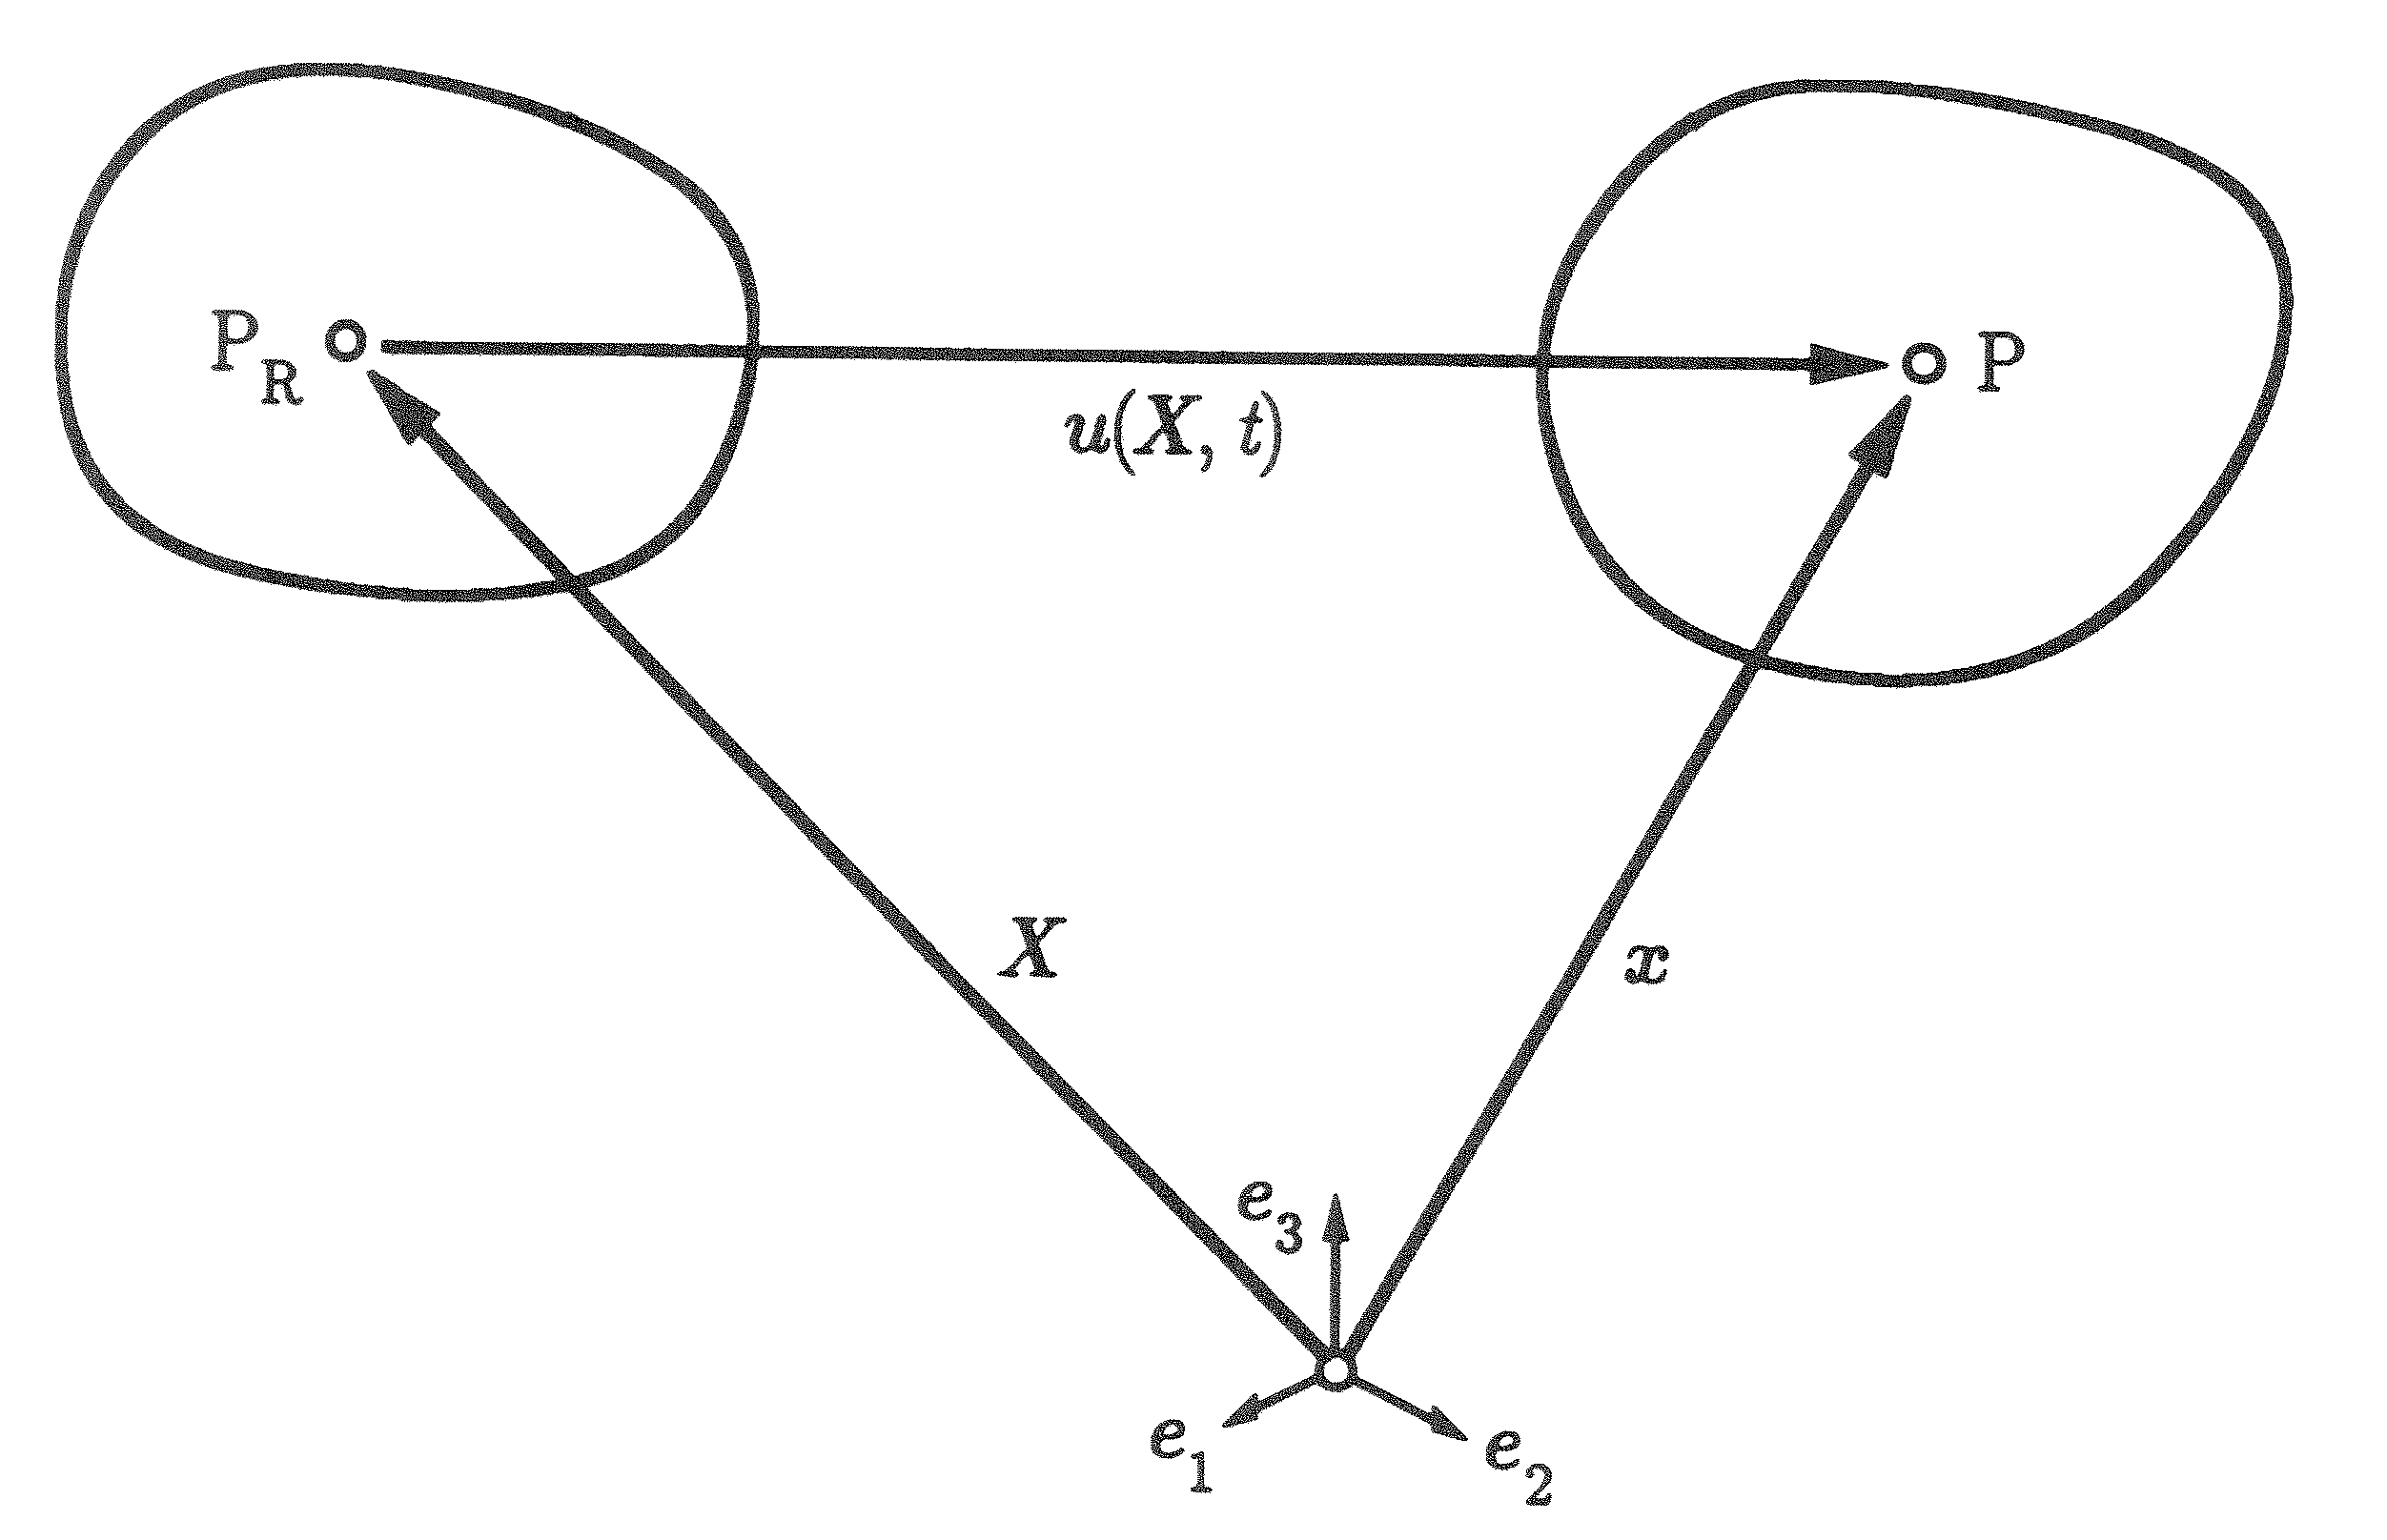
\includegraphics[width=0.7\textwidth]{figures/disp_vect.eps}
\caption{Definition of the displacement vector as the difference of the position vectors $\mathbf{x}$ and $\mathbf{X}$ of a material point (particle) of the body under consideration at various time $t$ (current time) and $t_0$ \cite{Haupt:2002}}
\label{fig:disp_vect}
\end{center}
\end{figure}

One of the primary variables within the context of the numerical simulation of coupled THM processes is the displacement vector $\mathbf{u}$ of the solid phase. The displacement vector is a commonly used kinematic variable to describe the motion (rigid body motion and/or deformation) of a solid material, and quantifies the change in the position of a given material point (cf. Fig.~\ref{fig:disp_vect}).
\begin{equation}
\mathbf{u}(\mathbf{X},t)\,=\,\mathbf{x}(\mathbf{X},t)\,-\,\mathbf{X}
\label{eq:defvec}
\end{equation}
In other words: the displacement vector connects the current position $\mathbf{x}$ of a material point which under the impact of external forces has been moved, and was located at time $t_0$ at the position $\mathbf{X}$. As, in general, the displacement vector will vary locally and temporally, $\mathbf{u}(\mathbf{X},t)=\mathbf{u}(\mathbf{X}(\mathbf{x},t),t)=\bar{\mathbf{u}}(\mathbf{x}{}{},t)\equiv\mathbf{u}$ represents a vector field as function of space and time.

For the sake of the possible comparison of the response of material bodies, which are composed of different materials and/or have a different geometry, to the impact of external forces it is not reasonable to deal with the physically obvious variables displacement and force, but rather to introduce relative physical variables like strain and stress measures. Strain measures represent second-order kinematic tensor variables characterizing the local deformation processes, which deviate from the rigid body motion of a material body.

Based on the definition of the displacement gradient
\begin{equation}
\nabla{\bar{\mathbf{u}}}(\mathbf{x},t)\,=\,\frac{\partial u_i}{\partial x_j}\,\miu{e}{i}{}\otimes\miu{e}{j}{}
\label{eq:dispgrad}
\end{equation}
with the orthonormal system of Cartesian base vectors $\miu{e}{i}{}$ ($i=1,2,3$), the strain tensor $\miu{\varepsilon}{}{}(\mathbf{x},t)$ in case of small (infinitesimal) deformations is established as the symmetric part of the displacement gradient.
\begin{equation}
\miu{\varepsilon}{}{}(\mathbf{x},t)\,=\,\frac{1}{2}
\left(\nabla{\bar{\mathbf{u}}}(\mathbf{x},t)\,+\,\left(\nabla{\bar{\mathbf{u}}}(\mathbf{x},t)\right)^{\mathrm{T}}\right)
\label{eq:straintens}
\end{equation}

The matrix of the coefficients of the strain tensor consists of so-called normal components
\begin{equation}
\varepsilon_{ii}\,=\,\frac{\partial u_i}{\partial x_i}
\label{eq:straintensnormal}
\end{equation}
and shear components.
\begin{equation}
\varepsilon_{ij}\,=\,
\frac{1}{2}\left(\frac{\partial u_i}{\partial x_j}\,+\,\frac{\partial u_j}{\partial x_i}\right)
\qquad(i\neq{j})
\label{eq:straintensshear}
\end{equation}
For special cases it can be easily shown that normal strain is geometrically interpreted as elongation of material line elements (Fig.~\ref{fig:extension}),
\begin{figure}[htb!]
\begin{center}
\footnotesize
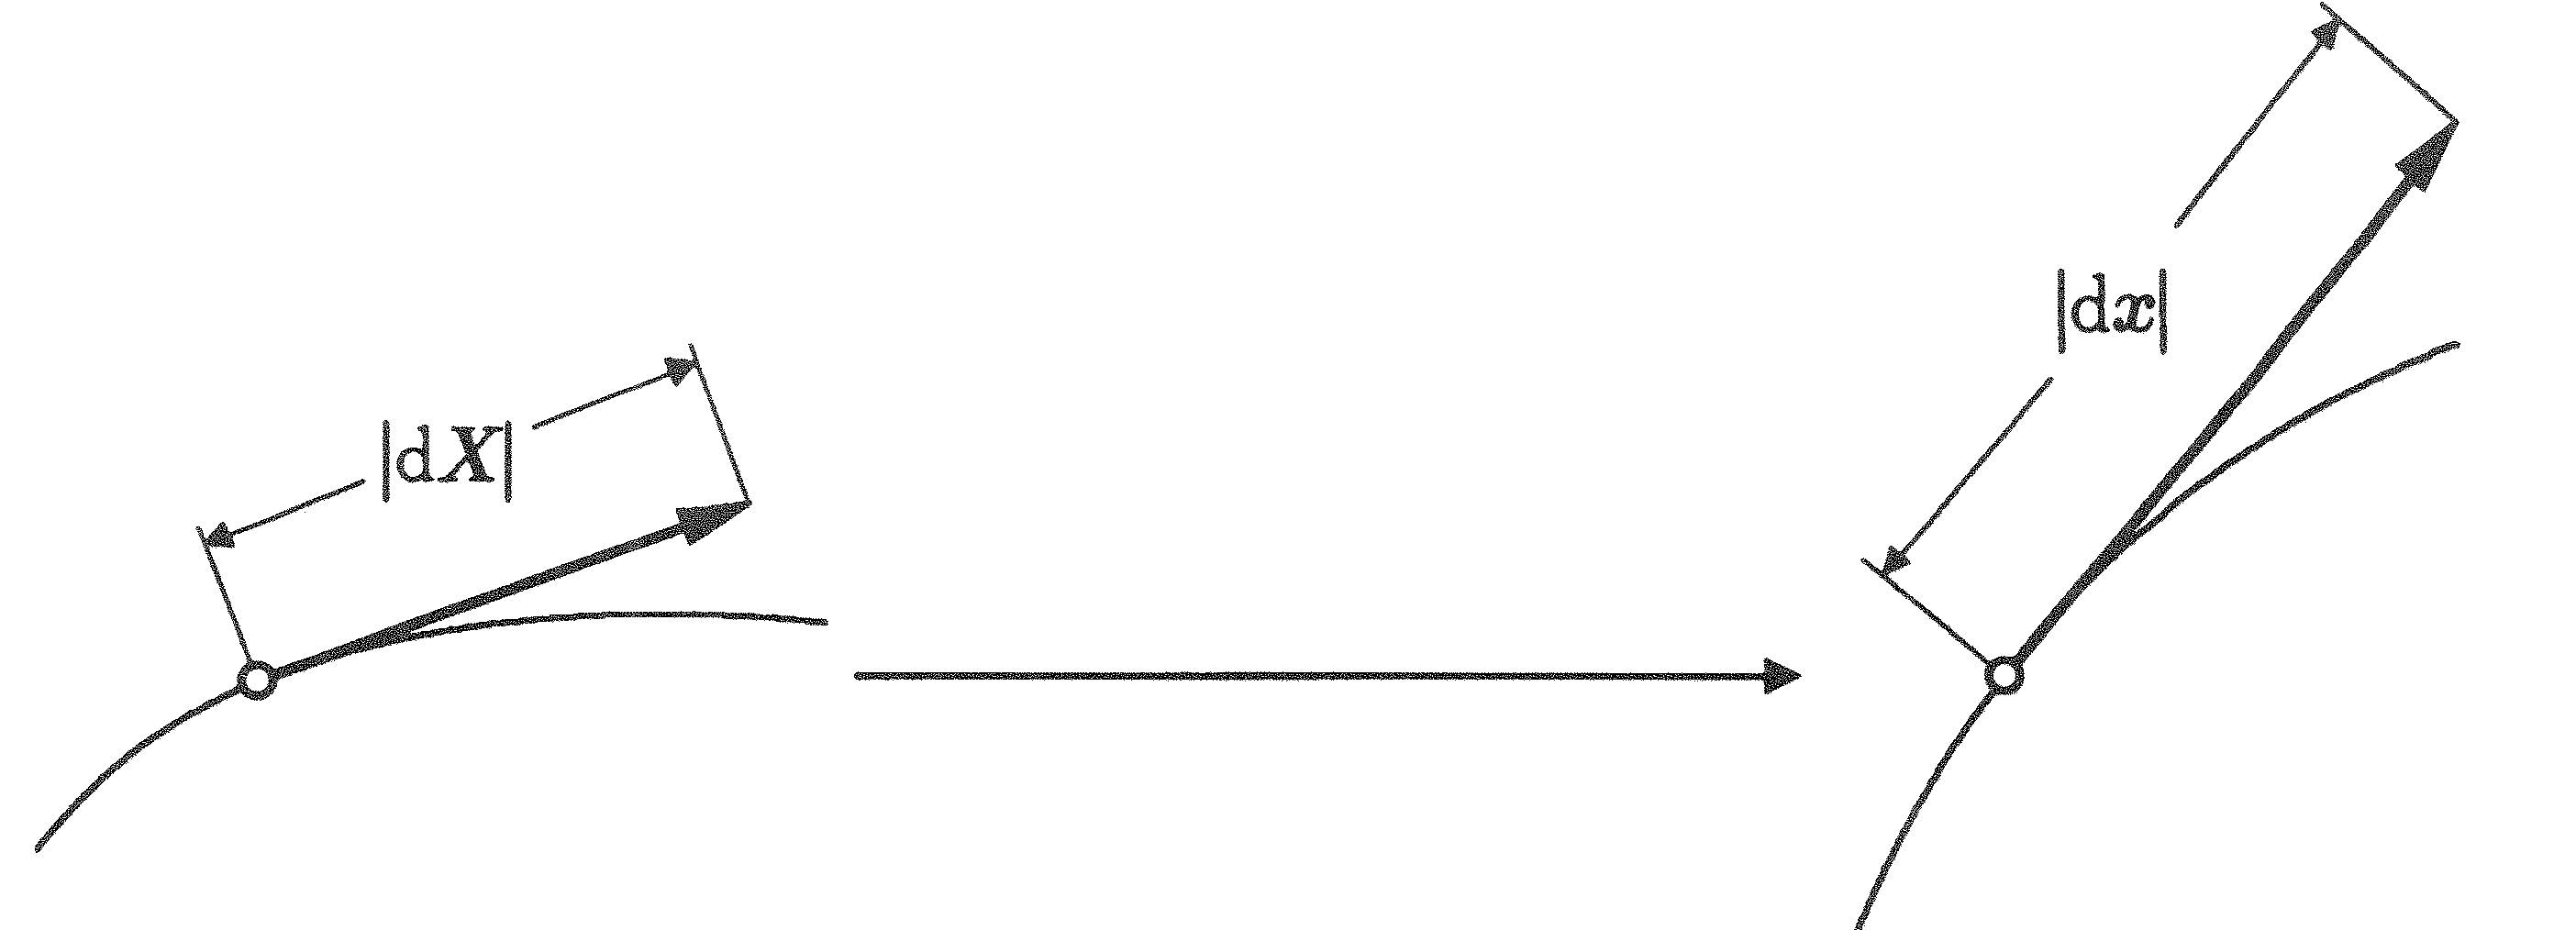
\includegraphics[width=0.7\textwidth]{figures/extension.eps}
\caption{Extension (normal strain) of a material line element $d\mathbf{X}=\vert d\mathbf{X}\vert\miu{e}{}{}$
\cite{Haupt:2002}}
\label{fig:extension}
\end{center}
\end{figure}

and shear strain represents the change of the angle between two material line elements, which initially were perpendicular to each other (Fig.~\ref{fig:shear}).
\begin{figure}[htb!]
\begin{center}
\footnotesize
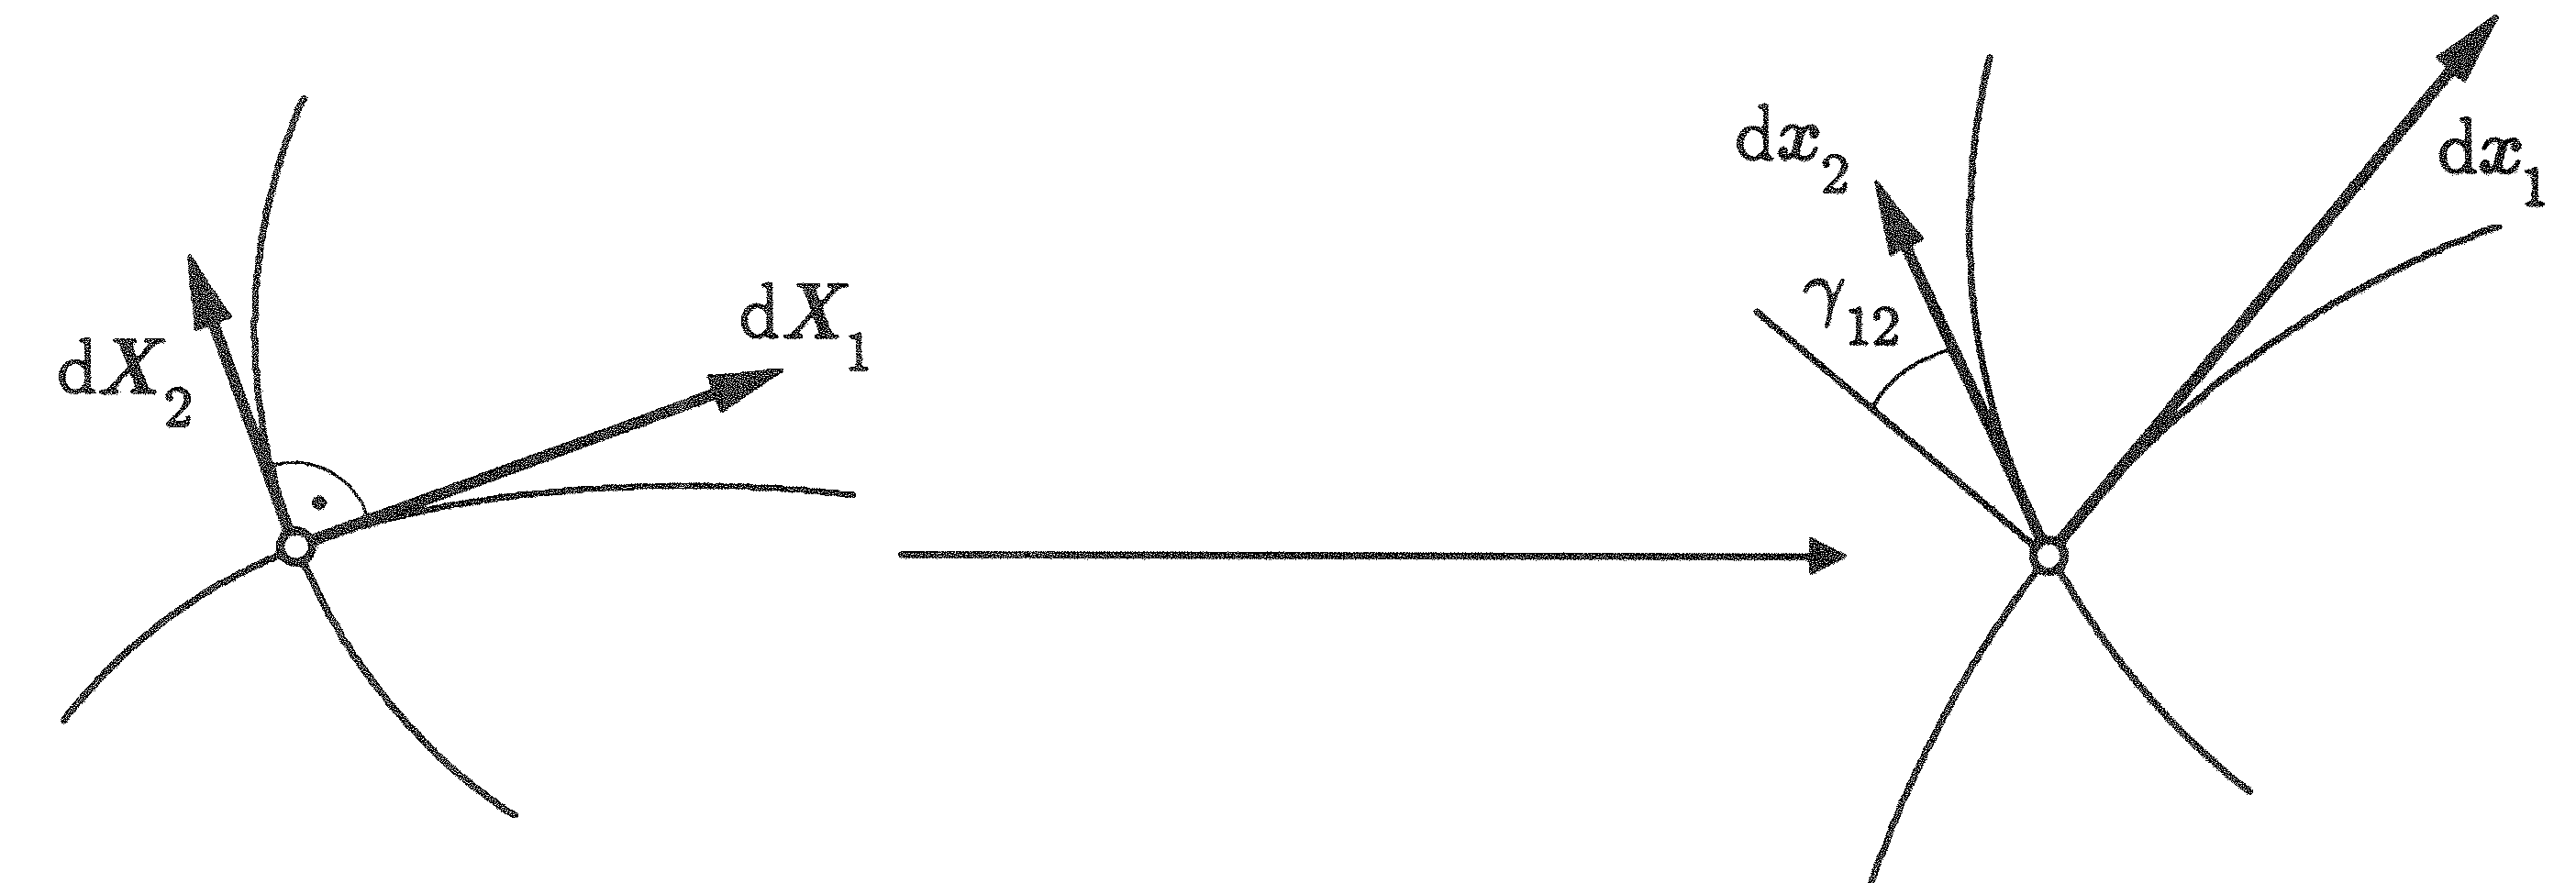
\includegraphics[width=0.7\textwidth]{figures/shear.eps}
\caption{Shear (shear strain) of two material line elements $d\mathbf{X}_1=\vert d\mathbf{X}_1\vert\miu{e}{1}{}$ and $d\mathbf{X}_2=\vert d\mathbf{X}_2\vert\miu{e}{2}{}$, which are orthogonal in the undeformed state \cite{Haupt:2002}}
\label{fig:shear}
\end{center}
\end{figure}

For the analysis of certain deformation processes it is reasonable to consider local volume changes and shape changes separately. Within this context, the strain tensor can be additively split into two parts: a volumetric $\miu{\varepsilon}{v}{}$ and a so-called deviatoric (volume-preserving) $\miu{\varepsilon}{d}{}$ one.
\begin{equation}
\miu{\varepsilon}{}{}\,=\,\miu{\varepsilon}{d}{}\,+\,\miu{\varepsilon}{v}{}
\label{eq:strainsplit}
\end{equation}
The individual partial strain tensors are defined as follows:
\begin{eqnarray}
\miu{\varepsilon}{v}{} & = & \frac{1}{3}\mathrm{tr}(\miu{\varepsilon}{}{})\,\mathbf{I}\,=\,
\frac{1}{3}(\varepsilon_{11}+\varepsilon_{22}+\varepsilon_{33})\,\mathbf{I}
\label{eq:devstrain}
 \\[2.0ex]
\miu{\varepsilon}{d}{} & = & \miu{\varepsilon}{}{}\,-\,\miu{\varepsilon}{v}{}
\label{eq:volstrain}
\end{eqnarray}

Based on the definition
\begin{equation}
\mathbf{v}^s(\mathbf{x},t)\,=\,\mathop{\bar{\mathbf{u}}}\limits^{\miu{.}{}{}}(\mathbf{x},t)
\label{eq:solidveloc}
\end{equation}
of the velocity of material points of the solid skeleton, the strain rate tensor
\begin{equation}
\miu{\varepsilon}{}{\dot}(\mathbf{x},t)\,=\,\mathbf{d}(\mathbf{x},t)\,=\,\frac{1}{2}
\left(\nabla\mathbf{v}^s(\mathbf{x},t)\,+\,\left(\nabla\mathbf{v}^s(\mathbf{x},t)\right)^{\mathrm{T}}\right)
\label{eq:strainratetens}
\end{equation}
with its coefficients
\begin{equation}
d_{ij}\,=\,
\frac{1}{2}\left(\frac{\partial v^s_i}{\partial x_j}\,+\,\frac{\partial v^s_j}{\partial x_i}\right)
\label{eq:strainratecoeff}
\end{equation}
can be defined, which is necessary for the investigation of deformation processes in case of rate-dependent material behavior.

In case of small strains, which was assumed here, the relation between the strain tensor and the displacement vector is a linear one (see section (\ref{eq:straintens})). Considering large strains, the definition of appropriate strain measures requires more sophisticated reflections about the kinematics of motion. As a result, different strain tensors can be obtained representing non-linear functions of the displacement vector. 

%-------------------------------------------------------------------------
\subsection{Stress Tensor}
\label{sec:stresstensor}

The momentum as well as the moment of momentum of a material body are affected by external forces acting on it, which represent the mechanical effect of the surroundings (cf. Fig.~\ref{fig:ext_forces}). Summarizing all local forces, the resultant force $\mathcal{F}$ can be defined.
\begin{equation}
\mathcal{F}\,=\,
\int\limits_{\partial\mathcal{B}}\mathbf{t}\,da\,+\,\int\limits_{\mathcal{B}}\mathbf{f}\,dm\,=\,
\int\limits_{\Gamma}\mathbf{t}(\mathbf{x},t,\mathbf{n})\,d\Gamma\,+\,
\int\limits_{\Omega}\mathbf{f}_v(\mathbf{x},t)\,\varrho(\mathbf{x},t)\,d\Omega
\label{eq:result_force}
\end{equation}
Generally, the material body under consideration bears forces distributed over its surface with the surface force
density $\mathbf{t}$ (traction, Cauchy stress vector), and forces distributed over the volume of the material body with the volume force density (mass distributed specific volume force) $\mathbf{f}_v$. As mentioned above, only gravity $\varrho\mathbf{g}$ should be considered as specific volume force.

\begin{figure}[htb!]
\begin{center}
\footnotesize
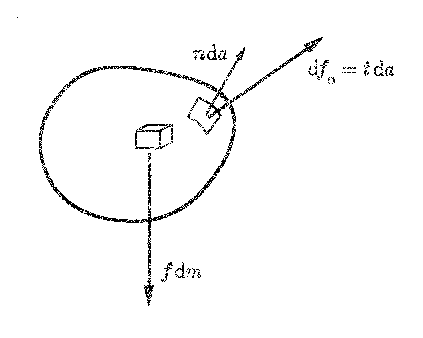
\includegraphics[width=0.6\textwidth]{figures/ext_forces.eps}
\caption{External volume and surface forces acting on infinitesimal geometrical elements of a material body \cite{Haupt:2002}}
\label{fig:ext_forces}
\end{center}
\end{figure}

The traction vector $\mathbf{t}(\mathbf{x},t,\mathbf{n})$ is considered to be a function of the location of its action on the surface, a function of time and of the normal vector, which characterizes the orientation of the surface element $d\miu{\Gamma}{}{}$. Assuming a linear relation between the traction and the normal vector (Cauchy's theorem), the stress measure $\miu{\sigma}{}{}(\mathbf{x},t)$ (Cauchy stress tensor) is defined as a link between surface traction and surface orientation. 
\begin{equation}
\mathbf{t}(\mathbf{x},t,\mathbf{n})\,=\,\miu{\sigma}{}{}(\mathbf{x},t)\,\mathbf{n}
\qquad\Rightarrow\qquad
\miu{\sigma}{}{}\,=\,\sigma_{ij}\,\miu{e}{i}{}\otimes\miu{e}{j}{}
\label{eq:cauchy_theorem}
\end{equation}
Based on Cauchy's theorem, the differential surface force $d\mathbf{f}_0$ acting on a surface element can be obtained. 
\begin{equation}
d\mathbf{f}_0\,=\,\mathbf{t}\,d\Gamma\,=\,(\miu{\sigma}{}{}\,\mathbf{n})\,d\Gamma\,=\,
\miu{\sigma}{}{}\,(\mathbf{n}\,d\Gamma)\,=\,\miu{\sigma}{}{}\,d\miu{\Gamma}{}{}
\label{eq:differ_surforce}
\end{equation}

For certain cases it is reasonable to use the so-called Kirchhoff stress tensor $\miu{\tau}{}{}$, a weighted Cauchy stress measure, instead of the Cauchy stress tensor itself.
\begin{equation}
\miu{\tau}{}{}\,=\,\frac{\varrho_0}{\varrho}\,\miu{\sigma}{}{}
\end{equation}

The second-order stress tensor characterizes the local internal load state referring to a material point of the body under consideration. Generally, it can be defined by three stress vectors acting on three faces of an infinitesimal tetrahedron, which are perpendicular to each other analyzing the equilibrium of forces for this domain. The coefficients of the resulting stress tensor are denoted by two indices -- the first indicates the direction of the normal vector of the face under consideration, the second one the direction of the stress coefficient (see Fig.~\ref{fig:stresstens_plane} for the three-dimensional case).

%\begin{figure}[htb!]
%\begin{center}
%\footnotesize
%\includegraphics[width=0.6\textwidth]{figures/cauchy_law.png}
%\caption{Equilibrium of surface tractions acting on the edges of an infinitesimal triangular element. Definition of %the Cauchy stress tensor using Cauchy's theorem (Jaeger et al. \cite{JCZ:2007})}
%\label{fig:cauchy_law}
%\end{center}
%\end{figure}

\begin{figure}[htb!]
\begin{center}
\footnotesize
%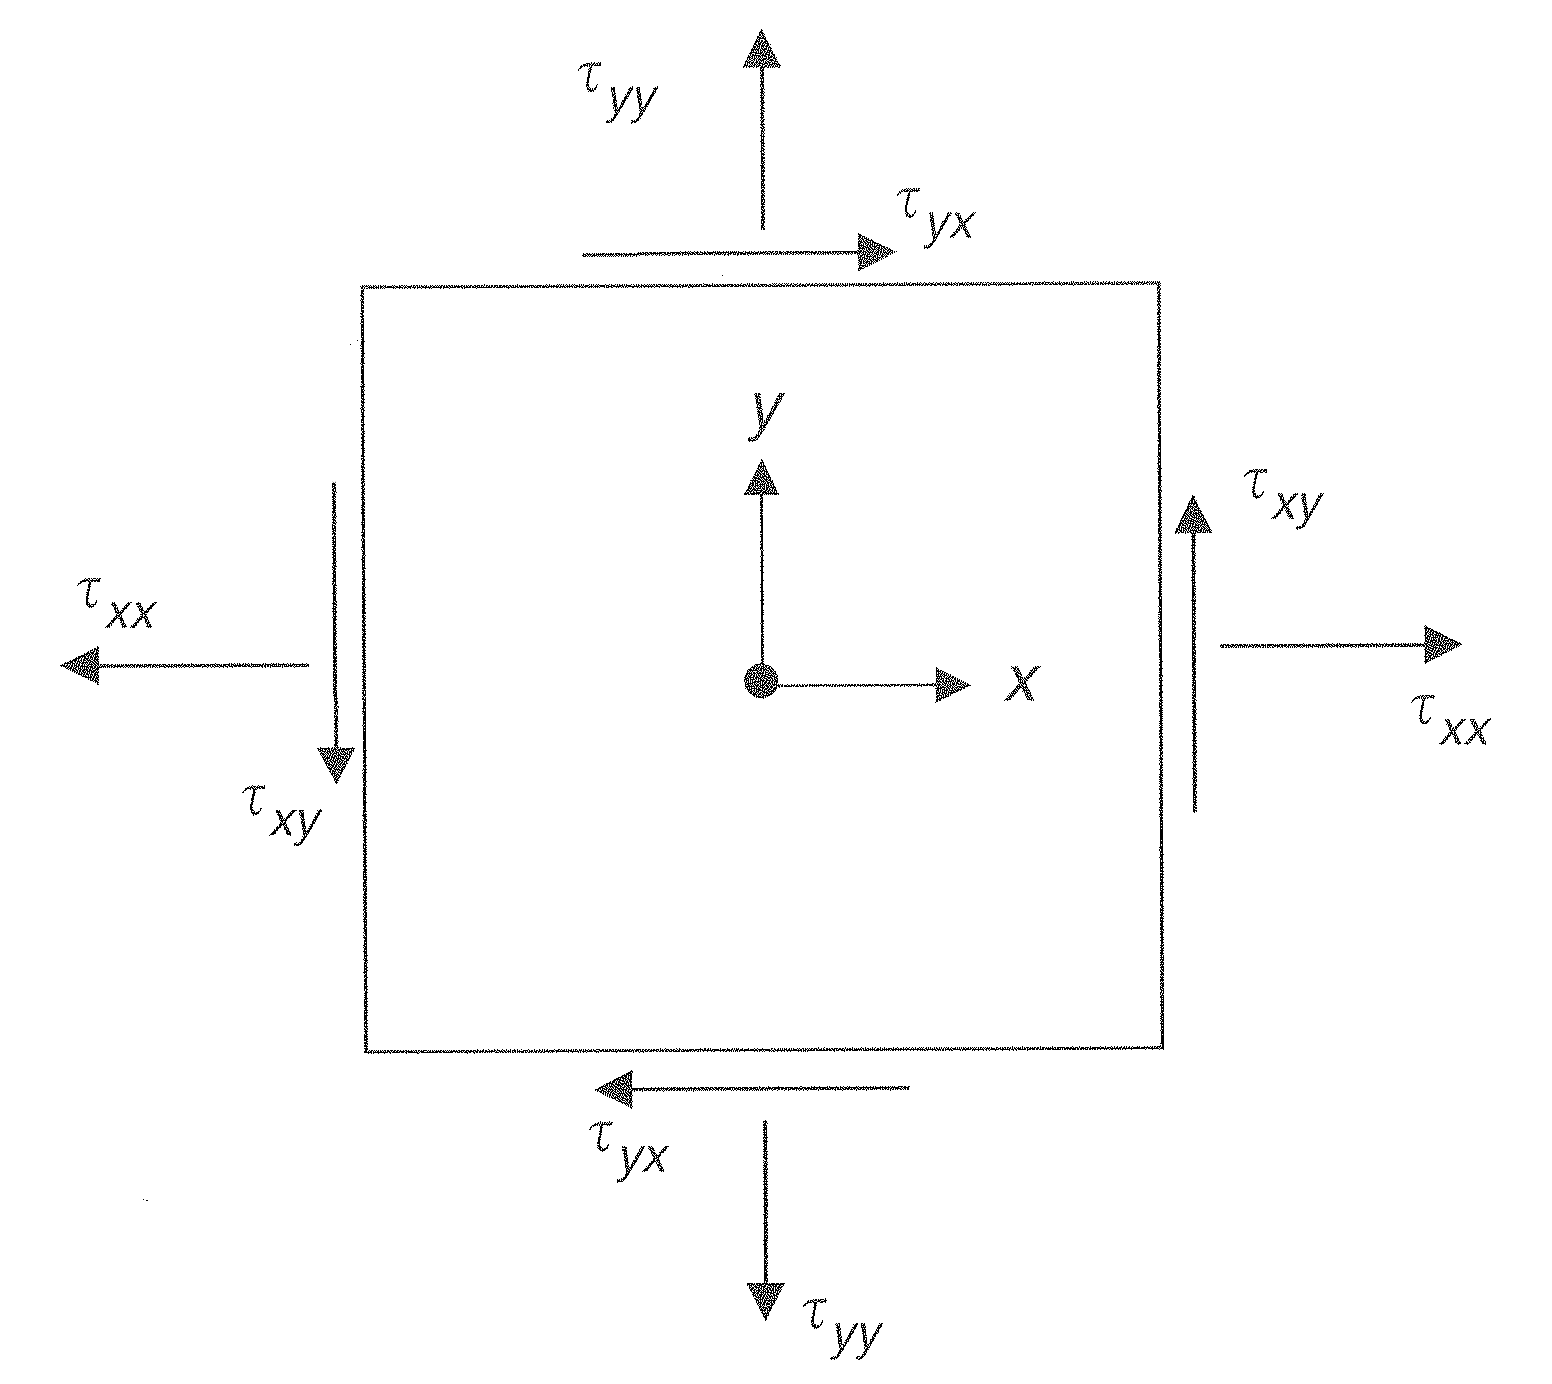
\includegraphics[width=0.6\textwidth]{figures/stresstens_plane.eps}
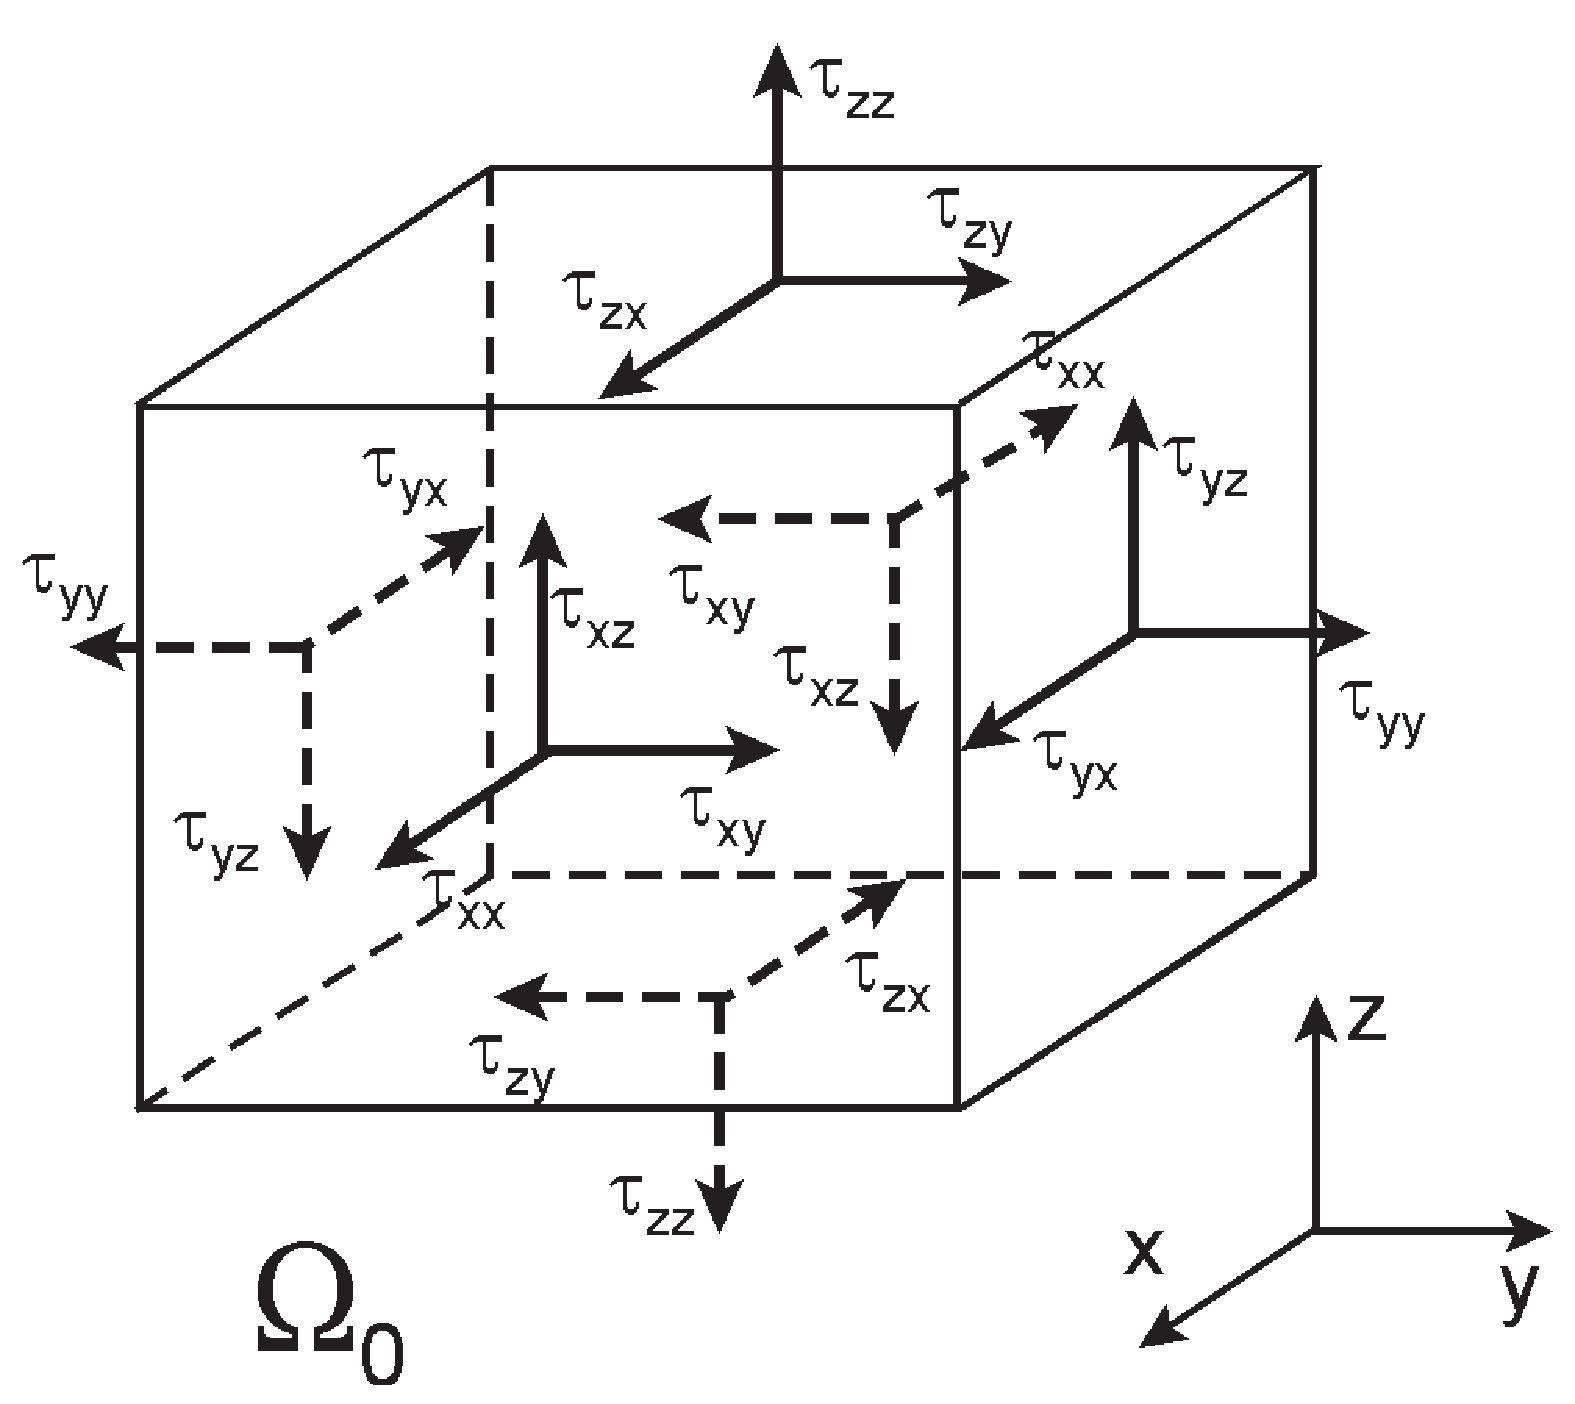
\includegraphics[width=0.6\textwidth]{figures/mech5.eps}
\caption{Coefficients of the stress tensor acting on a small hexahedral element \cite{Kol:02}}
\label{fig:stresstens_plane}
\end{center}
\end{figure}

The sign convention, usually applied in continuum mechanics, implies positive stress coefficients coinciding with the directions of the axes of coordinates at faces with normal vectors also coinciding with the directions of the axes of ccordinates. Consequently, tensile stress coefficients are positive, compressive stresses negative. Positive stress coefficients on opposite faces are oppositely directed (but of equal absolute value). The matrix of the coefficients of the (Kirchhoff) stress tensor is composed as follows:
\begin{equation}
\tau_{ij}\,=\,
\left(
\begin{array}{ccc}
\tau_{xx} & \tau_{xy} & \tau_{xz} \\
\tau_{yx} & \tau_{yy} & \tau_{yz} \\
\tau_{zx} & \tau_{zy} & \tau_{zz}
\end{array}
\right)
\label{eq:stress_matrix}
\end{equation}
Analogous to the strain tensor, the coefficients $\tau_{xx},\,\tau_{yy},\,\tau_{zz}$ are called normal stresses, the coefficients $\tau_{ij}\quad(i\neq j)$ shear stresses with $\tau_{ij}=\tau_{ji}$ (symmetry of the stress tensor, which results from the balance of moment of momentum).

In the special uniaxial stress case only at one face of a volume element a normal stress occurs, whereas all the other faces are stress-free. Consequently, the stress coefficient is calculated as the force acting on the face under consideration divided by its area.








%-------------------------------------------------------------------------
\subsection{Conservation principles}
\label{sec:conservation_principles}
%\section{Conservation principles}

\footnote{Truesduell}

Based on the kinematical foundation (section \ref{sec:kinematics}) we formulate the general conservation principle of continuum mechanics for both Eulerian and Lagrangian points of view (section \ref{sec:euler_lagrange}).
%
The amount of a (conservation) quantity in a defined volume $\Omega$ is given by

\begin{eqnarray}
\Psi =
\int\limits_\Omega \psi d\Omega(t)
\end{eqnarray}

where $\Psi$ is an extensive conservation quantity\index{quantity
- extensive } (i.e. mass, momentum, energy) and $\psi$ is the
corresponding intensive conservation quantity\index{quantity -
intensive} such as mass density $\rho$, momentum density $\rho \bf
v$ or energy density $e$ (see Table
\ref{tab:conservation_quantities}).

%
\begin{table}[htb!]
\caption{Conservation quantities}
\label{tab:conservation_quantities}
\begin{center}
\begin{tabular}{|ll|ll|}
\hline
Extensive  quantity &  Symbol    &  Intensive quantity      &  Symbol  \\
\hline \hline
%\mbox{\rule[1mm]{0cm}{3mm}Mass}
Mass                &  $M$,$M_k$ & Mass density             & $\rho$,$\rho_k$  \\
Linear momentum     &  $\bf m$   & Linear momentum density  & $\rho \bf v$ \\
Energy              &  $E$       & Energy density           & $e = \rho i + \frac 1 2 \rho v^2 $
\\[1pt]
\hline
\end{tabular}
\end{center}
\end{table}
%

The balance equations for mass, momentum and energy conservation can be derived based on two fundamental principles, i.e. Eulerian and Lagrangian frameworks (e.g. \cite{Kol:02})
%
Both conservation principles are related by two different forms of derivatives
\begin{equation}
\frac{d \psi}{dt}
=
\frac{\p \psi}{\p t} + \v\cdot\nabla\psi
\label{eqn:derivatives}
\end{equation}
the total (or material) $d$ and partial derivatives $\p$, respectively.
%
The general integral balance equation is given by
%
\begin{eqnarray}
\frac{d}{dt} \int\limits_\Omega \psi~d\Omega
=
\int\limits_\Omega
\left(
\frac{\partial\psi}{\partial t}
+
\nabla \cdot {\mathbf{\Phi}}
\right)
d\Omega
=
\int\limits_\Omega q^\psi d\Omega
\label{eqn:general_balance_equation}
\end{eqnarray}
%
where $\psi$ is a general conservation quantity, $\mathbf{\Phi}$ is the total flux of $\psi$, and $Q$ is a source/sink term for $\psi$.
%
The corresponding extensive and intensive conservation quantities are summarized in Tab. \ref{tab:conservation_quantities}.

The total flux ${\bf\Phi}^\psi$ of a quantity $\psi$ is defined as
\begin{eqnarray}
{\bf\Phi}^\psi
=
{\bf v}^E \psi
\end{eqnarray}

where ${\bf v}^E$ is a mean particle velocity\index{quantity - velocity -
particle}. Physically ${\bf\Phi}^\psi$ represents the quantity of
$\psi$ passing through a unit area of the continuum, colinear with
${\bf v}^E$, per unit time with respect to a fixed coordinate
syste, i.e. Eulerian point of view.

For the case of a multi-component continuum let ${\bf v}$ denote
the mass-weighted velocity\index{quantity - velocity - mass-weighted}
describing a more ordered motion of the particles of a fluid
element. The total flux can be written as
\begin{eqnarray}
{\bf\Phi}^\psi
=
{\bf v}^E \psi
=
\underbrace{{\bf v} \psi}_{{\bf\Phi}^\psi_A}
+
\underbrace{({\bf v}^E-{\bf v}) \psi}_{{\bf\Phi}^\psi_D}
\end{eqnarray}

and, therefore, decomposed into two parts: an advective flux
${\bf\Phi}^\psi_A$ and a diffusive flux ${\bf\Phi}^\psi_D$
relative to the mass-weighted velocity:

\begin{itemize}
 \item
Advective flux\index{flux - advective} of quantity $\psi$
\begin{eqnarray}
{\bf\Phi}^\psi_A
=
{\bf v}\psi
\end{eqnarray}

 \item
Diffusive flux\index{flux - diffusive} of quantity $\psi$
(Fick's law)\index{law - Fick}
\begin{eqnarray}
{\bf\Phi}^\psi_D=
-\alpha \nabla\psi
\end{eqnarray}
\end{itemize}

where $\alpha$ is a diffusivity coefficient. The negative sign indicates, that diffusive flux is positive in the direction of negative gradient.

If the conservation quantity is a vector (e.g. linear momentum)
then the flux becomes a tensor and the source term a vector (e.g. body forces):

\begin{itemize}

\item Advective flux of vector quantity $\psi$
%
\begin{eqnarray}
{\bf\Phi}^\psi_A
=
% {\bf v}:{\Boldmath\psi}
{\bf v}:{\mathbf{\psi}}
=
\left[
\begin{array}{ccc}
v_x & v_y & v_z
\end{array}
\right]
\left[
\begin{array}{c}
\psi_x \\ \psi_y \\ \psi_z
\end{array}
\right]
=
\left|
\begin{array} {lll}
v_x \psi_x &  v_x \psi_y & v_x \psi_z \\
v_y \psi_x &  v_y \psi_y & v_y \psi_z \\
v_z \psi_x &  v_z \psi_y & v_z \psi_z
\end{array}
\right|
\end{eqnarray}

\item Diffusive flux of vector quantity $\psi$
%
\begin{eqnarray}
{\bf\Phi}^\psi_D
=
% -\rho \nabla:{\Boldmath\psi}
-\rho \nabla:{\mathbf{\psi}}
=
-\alpha
\left|
\begin{array} {lll}
\frac{\partial\psi_x}{\partial x} & \frac{\partial\psi_y}{\partial y} & \frac{\partial\psi_z}{\partial z} \\
\frac{\partial\psi_x}{\partial x} & \frac{\partial\psi_y}{\partial y} & \frac{\partial\psi_z}{\partial z} \\
\frac{\partial\psi_x}{\partial x} & \frac{\partial\psi_y}{\partial y} & \frac{\partial\psi_z}{\partial z}
\end{array}
\right|
\end{eqnarray}
\end{itemize}

When substituting the flux definition into the general balance equation (\ref{eqn:general_balance_equation}),
we yield the so-called transport equation

\begin{eqnarray}
\frac{d}{dt} \int\limits_\Omega \psi~d\Omega
=
\underbrace{\int\limits_\Omega \frac{\partial\psi}{\partial t}~d\Omega}_{1}
+
\underbrace{\int\limits_\Omega \nabla \cdot ({\bf v}\psi)~d\Omega}_{2}
-
\underbrace{\int\limits_\Omega \nabla \cdot (\alpha\nabla\psi)~d\Omega}_{3}
=
\underbrace{\int\limits_\Omega q^\psi}_{4}
\label{eqn:integral_balance_equation}
\end{eqnarray}

with the followind terms:

\renewcommand{\arraystretch}{0.9}
\begin{enumerate}
 \item Rate of increase of $\psi$ within a fluid element
 \item Net rate of $\psi$ due to flux out of the fluid element
 \item Rate of increase / decrease of $\psi$ due to diffusion
 \item Rate of increase / decrease of $\psi$ due to sources
\end{enumerate}

%-------------------------------------------------------------------------
\section{Porous medium}
\label{sec:porous_medium}
%\section{Porous medium}

Soil or rock can be considered as a multiphase medium consisting
of a solid phase (solid matrix) and of one or more fluid phases
(gas and liquids), which occupy the void space (Fig.
\ref{fig:porous_medium}). Fluids are immiscible\index{fluid -
immiscible}, if a sharp interface is maintained between them. In
general, a phase is defined as a part of a continuum, which is
characterized by distinct material properties and by a
well-defined set of thermodynamic state variables. State variables
describe the physical behaviour at all points of the phase. They
must vary continuously within the considered phase of a continuum.
Phases are separated from each other by surfaces referred to as
interphase boundaries. Transport of components may occur within a
phase and/or across interphase boundaries. Those
interphasic\index{process - interphase} exchange processes between
adjacent phases can result from diffusive and/or advective
mechanisms.

In fact, it is impossible to describe the complex geometry of the
solid matrix and the topology of the void space at the microscopic
level, i.e. the topology of the pore space will never be known in
detail. As a consequence, boundary conditions for a mathematical
model cannot be stated at this scale, since they are not known at
the microscopic level. Moreover, it will be extremely difficult to
measure values of state variables at each point within a phase in
order to observe processes, to calibrate and to verify any model.
Finally, the complete formulation and resolution of balance
equations at the microscopic\index{scale - microscopic} level is
impossible and may not be reasonable. Therefore, it is necessary
to transform the problem from a microscopic scale to a
macroscopic\index{scale - macroscopic} level. Starting from the
microscopic balance equations for extensive quantities (masses,
momentum, energy), this procedure is the subject of the theory of
the porous medium 
\cite{Bea:72,Die:85,Ehl:89,BeaBac:90,Kin:1992,Hel:97,LewSch:98,Boe:00}
%(Bear 1972, Diersch 1985, Bear \& Bachmat 1990, de Boer \& Ehlers 1986, Lewis \& Schrefler 1998, de Boer 2000).
The entire problem is rewritten in terms of averages of
microscopic quantities, which have measurable values. The
resulting macroscopic model is referred to as the continuum
approach\index{model - continuum}. This conceptual model implies
that a real system is replaced by a number of overlapping continua
representing the corresponding phases. It is assumed that each
phase, occupying a certain part of the porous domain, is regarded
as a continuum. These individual phases interact with each other
at any place within the entire domain, because they are present at
each point within the porous medium, i.e. all phases are
completely mixed.
%
\begin{eqnarray}
\Omega_0
=
\sum_{\alpha} \Omega^\alpha
\end{eqnarray}
%
In addition to the porous medium approach, there exist different
types of structural models for fractured rocks, which characterize
the degree of inhomogeneity: the fractured medium\index{medium -
fractured} and the fractured porous medium\index{medium - porous
fractured}. The term fractured medium means that only the
fractures are important for the considered process, so blocks
surrounded by the fractures may be neglected in the model. The
term fractured porous medium means that both fracture system and
porous matrix are significant for the considered process. The
domain of a fractured porous medium consists of two subdomains,
representing heterogeneities at different scales, i.e. the
diameter of pores in the matrix and the characteristic length of
fractures.

Appropriate averaging rules must be defined in order to realize
the above described transformation from a microscopic to a
macroscopic level. For this purpose, a well-defined sample size of
an averaging volume must be found, which is referred to as the
representative elementary volume\index{volume - representative
elementary} (abbreviated REV). On the one hand, this averaging
unit has to be sufficiently large, so that the influence of
microscopic inhomogeneity on the values of averaged (macroscopic)
quantities will vanish, i.e. they become independent of size,
shape, and orientation of the REV. On the other hand, the REV must
be small enough to reflect the macroscopic heterogeneity. In
particular, the REV must be much smaller than the domain of
interest, which may vary in size for a flow or a transport
problem, respectively. From the mathematical point of view, the
macroscopic (averaged) quantities must be continuous and
differentiable functions (in space and in time), so that solutions
of the governing differential balance equations can be determined.
Finally, the continuum approach cannot be employed unless a common
range of a REV can be selected for all material properties (e.g.
porosity, permeability, dispersivity) as well as for all relevant
state variables. This requirement is important with respect to the
different conceptual models for fractured rock, which are
introduced in the following.

%=7.2==============================================================================
\subsection{Macroscopic Equations}

%\subsubsection*{Statistic approach}
%\index{model - statistic}

In fact, it is impossible to describe the complex geometry of the solid matrix
and the topology of the void space at the microscopic level, i.e. the topology
of the pore space will never be known in detail. Therefore, a statistical
approach is used for the derivation of balance equations at a macroscopic
level. The physical property of a porous medium is decomposed in phase-related
mean values $\overline{\psi^\alpha}$ and local fluctuations ${\psi'}^\alpha$.
%
\begin{eqnarray}
\psi^\alpha
=
\overline{\psi^\alpha}
+
{\psi'}^\alpha
\end{eqnarray}

%\subsubsection*{Averaging volume}
%\index{scale - averaging - volume}

An appropriate averaging volume is called
the Representative Elementary Volume (REV) (Fig. \ref{rev}).

% *** EPS-Grafik ***
\begin{figure}[htb!]
\begin{center}
\footnotesize
%\psfrag{Synonym}[pos][pos]{Tex-Ersetzung}
%\psfrag{x}[][]{$t$}
%\psfrag{y}[b][t]{$y(t)$}
%\psfrag{t}[][]{ }
%\includegraphics[height=7.5cm,width=11cm]{../figures/fig_71.bmp}
\includegraphics[width=0.95\columnwidth]{figures/por2.eps}  % Filename.eps
\caption{Definition of the representative elementary volume (REV) \cite{BeaBac:90}} 
\label{rev}
\end{center}
\end{figure}
%

%\subsubsection*{Averaging operator}

Several averaging procedures can be defined \cite{BeaBac:90}. As
an example we consider volumetric averaging which is also denoted as the
concept of volume fractions. The volumetric averaging operator is given by
%
\begin{eqnarray}
\overline{\psi^\alpha}^\alpha
=
\frac{1}{\epsilon^\alpha \Omega_0}
\int\limits_{\Omega_0} f^\alpha \psi^\alpha d\Omega
\label{eqn:mean}
\end{eqnarray}

where $\alpha$ is the phase indicator, $\epsilon^\alpha =
\Omega^\alpha/\Omega_0$ is the volumetric fraction of the $\alpha$
phase, $\Omega_0$ is the averaging volume (corresponding to the
representative elementary volume), $f^\alpha=1/0$ (inside or
outside $\alpha$ phase) is the phase distribution function.

%\subsubsection*{Averaging rules}
%\index{scale - averaging - rules}

Due to the above definition the following averaging rules can be derived.

\begin{itemize}
 \item Sum
\begin{eqnarray}
\overline{\psi_1^\alpha+\psi_2^\alpha}
=
\overline{\psi_1^\alpha}+\overline{\psi_2^\alpha}
\end{eqnarray}

 \item Product
\begin{eqnarray}
\overline{\psi_1^\alpha \psi_2^\alpha}
=
\overline{\psi_1^\alpha}\,\overline{\psi_2^\alpha}
+
\overline{{\psi_1'}^\alpha {\psi_2'}^\alpha}
\end{eqnarray}

 \item Time derivative
\begin{eqnarray}
\epsilon^\alpha \overline{\frac{\partial \psi^\alpha}{\partial t}}
=
\frac{\partial \epsilon^\alpha \overline{\psi^\alpha}}{\partial t}
-
\frac{1}{\Omega_0}
\int\limits_{S^{\alpha\beta}}\psi^\alpha {\bf w} \cdot d{\bf S}
\end{eqnarray}

 \item Spatial derivative
\begin{eqnarray}
\epsilon^\alpha \overline{\nabla\psi^\alpha}
=
\nabla(\epsilon^\alpha\overline{\psi^\alpha})
+
\frac{1}{\Omega_0}
\int\limits_{S^{\alpha\beta}}\psi^\alpha \cdot d{\bf S}
\end{eqnarray}

\end{itemize}

where $\bf w$ is the velocity of the $\alpha\beta$-phase interface.

%\subsubsection*{General macroscopic balance equation}
%\index{equation - general balance}

To derive a phase related macroscopic balance equation,
we have to average the balance equation in differential form
for a certain phase (\ref{eqn:general_balance_equation}).
By use of the above averaging operators and rules
the following general macroscopic balance equation
can be obtained.
%
\begin{eqnarray}
\frac{\partial \epsilon^\alpha \overline{\psi^\alpha}}{\partial t}
=
-
\nabla\cdot(
\epsilon^\alpha\bar{\psi^\alpha}\overline{{\bf v}^\alpha}
+
\epsilon^\alpha\overline{{\psi'}^\alpha{\bf v'}^\alpha}
+
\epsilon^\alpha\overline{{\bf\Phi}_{\textrm{\tiny Diff}}^{\psi^\alpha}}
)
\nonumber \\
-
\frac{1}{\Omega_0}
\int\limits_{S^{\alpha\beta}} {\bf\Phi}_{\textrm{\tiny Diff}}^{\psi^\alpha} \cdot d{\bf S}
-
\frac{1}{\Omega_0}
\int\limits_{S^{\alpha\beta}}\psi^\alpha ({\bf v-w}) \cdot d{\bf S}
+
q^{\psi^\alpha}
\end{eqnarray}

with the dispersive flux
\begin{eqnarray}
{\bf\Phi}_{\textrm{\tiny Disp}}^{\psi^\alpha}
=
\epsilon^\alpha\overline{{\psi'}^\alpha{\bf v'}^\alpha}
\end{eqnarray}

%------------------------------
\subsection{Theory of Mixtures}
\label{sec:mixtures}

The Theory of Mixtures as one of the basic approaches to model the complex behavior of porous media has been developed over decades (concerning basic assumptions see e.g. \cite{Bow:1976,TT:1960}). As the Theory of Mixtures does not incorporate any information about the microscopic structure of the material\footnote{Within the context of the Theory of Mixtures the ideal mixture of all constituents of a multiphase medium is postulated. Consequently, the realistic modeling of the mutual interactions of the constituents is difficult.}, it has been combined with the Concept of Volume Fractions by e.g. \cite{Bow:1980,BE:1986a,LewSch:98,Pre:1980}. Within the context of this enhanced Theory of Mixtures (also known as Theory of Porous Media), all kinematical and physical quantities can be considered at the macroscale as local statistical averages of their values at the underlying microscale.
%
Concerning a detailed overview about the history of the modeling of the behavior of multiphase multicomponent porous media, the reader is referred to e.g. \cite{Boe:00}. Comprehensive studies about the theoretical foundation and numerical algorithms for the simulation of coupled problems of multiphase continua are given in e.g. \cite{Boe:00,EB:2002,LewSch:98} and the quotations therein. 

The individual constituents $\varphi^{\alpha}$ of a porous material represent the phases of the overall aggregate or components within a phase. Below, $\alpha=s$ marks one immiscible solid phase (no sorption processes are considered), and $\alpha=\gamma$ denote several immiscible pore fluid phases. 
%
A porous medium, however, consists of multiple phases (fluids such as water, air and non-aqueous phase liquids (NAPLs) as well as solids). 
Moreover, these phases can contain several chemical components which can be dissolved in liquids or adsorbed to the solid phase (Fig. \ref{fig:porous_medium}).

\newpage
.
\vspace{4cm}
\begin{figure}[htbp]
\hspace{3cm}
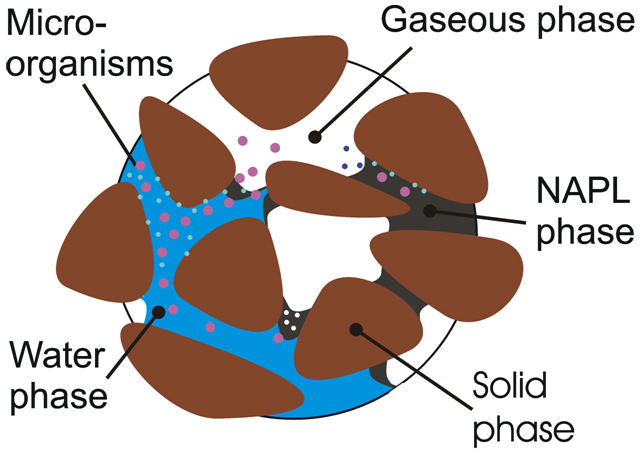
\includegraphics[width=0.06\columnwidth]{figures/pm}
\caption{Conceptual approach of a porous medium model, adopted from \cite{Kol:02}}
\label{fig:porous_medium}
\end{figure}

Within the framework of the Concept of Volume Fractions, scalar variables like volume fractions and saturations are defined to describe the microstructure of a porous medium in a macroscopic manner neglecting the real topology and distribution of the pores. These variables serve as measures of local fractions of the individual constituents. The volume fractions $n^{\alpha}$ represent the ratio of the partial volume $dv^{\alpha}$ of a given constituent $\varphi^{\alpha}$ of a multiphase body with respect to the overall volume $dv$ of a representative elementary volume (REV) of the control domain $\Omega$ under consideration. Consequently, based on the definitions of the overall volume of the control domain
\begin{equation}
V=\int\limits_{\Omega}\,dv
\label{eq1}
\end{equation}
and the corresponding partial volumes of the individual constituents
\begin{equation}
V^{\alpha}=\int\limits_{\Omega}\,dv^{\alpha}\qquad\mbox{with}\qquad V=\sum\limits_{\alpha}\,V^{\alpha}
\label{eq2}
\end{equation}
the volume fractions
\begin{equation}
n^{\alpha}=\frac{dv^{\alpha}}{dv}
\label{eq3}
\end{equation}
provide some information about the local volume distribution of the individual constituents.
\begin{equation}
V^{\alpha}=\int\limits_{\Omega}\,dv^{\alpha}=\int\limits_{\Omega}\,n^{\alpha}\,dv
\label{eq4}
\end{equation}
One of the most characteristic media properties of a porous material is the porosity, the local amount of fluid volume fractions.
\begin{equation}
n=\sum\limits_{\gamma}\,n^{\gamma}=1\,-\,n^s
\label{eq5}
\end{equation}
Since, in general, the overall medium is completely filled with matter, from Eqn.~(\ref{eq2}) follows the saturation condition regarding the overall aggregate.
\begin{equation}
\sum\limits_{\alpha}\,n^{\alpha}=1
\label{eq6}
\end{equation}

If multiphase flow occurs, it is more convenient for various applications to use the (partial) fluid saturations $S^{\gamma}$ instead of the volume fractions. These local functions are given by
\begin{equation}
S^{\gamma}=\frac{dv^{\gamma}}{dv-dv^s}=\frac{n^{\gamma}}{n}
\label{eq7}
\end{equation}
obviously fulfilling the saturation condition regarding the pore content.
\begin{equation}
\sum\limits_{\gamma}\,S^{\gamma}=1
\label{eq8}
\end{equation}

Usually, constraint conditions addressing real physical effects are formulated to simplify complex mathematical and numerical models. Within the context of porous media, it is reasonable in most applications to assume the (material) incompressibility of constituents as a substantial constraint condition. The issue of (in)compressibility of a material is closely connected to the possible temporal evolution of its mass density.

Within the framework of the Concept of Volume Fractions, two different formulations of mass density related to the constituents of a porous medium are introduced. The so-called material (effective, realistic) density $\rho^{\alpha R}$ is defined as the ratio of the mass fraction $dm^{\alpha}$ of the given individual constituent $\varphi^{\alpha}$ with respect to its partial volume fraction.
\begin{equation}
\rho^{\alpha R}=\frac{dm^{\alpha}}{dv^{\alpha}}
\label{eq9}
\end{equation}
In contrast, the so-called partial (global, bulk) density is given by the ratio of the mass fraction of the constituent under consideration with respect to the volume fraction of the overall aggregate.
\begin{equation}
\rho^{\alpha}=\frac{dm^{\alpha}}{dv}
\label{eq10}
\end{equation}
Based on the definition of the volume fractions (\ref{eq3}), the material and the partial densities are correlated to each other.
\begin{equation}
\rho^{\alpha}=n^{\alpha}\,\rho^{\alpha R}
\label{eq11}
\end{equation}
If the volume fractions change with time under external loading, from Eqn.~(\ref{eq11}) follows that for an intrinsically incompressible individual constituent (constant material mass density) compressibility referred to the overall aggregate is observed.
\begin{equation}
\rho^{\alpha R}=\mbox{const} \quad\Rightarrow\quad
\rho^{\alpha}\,\neq\,\mbox{const}\quad\mbox{as}\quad n^{\alpha}\,\neq\,\mbox{const}
\label{eq12}
\end{equation}

Obviously, the mass density of the porous medium (homogenized overall aggregate) is defined as the sum of the partial densities of its constituents.
\begin{equation}
\rho=\sum\limits_{\alpha}\rho^{\alpha}
\label{eq13}
\end{equation}

The conceptual idea behind the formulations and relations presented above consists in the assumption that the mass fractions of all constituents of the multiphase medium are simultaneously present and statistically uniformly distributed over the entire control domain. Within this context, the material body under consideration is theoretically substituted by an aggregate completely and continuously filled by superimposed (overlapping) homogenized partial continua. In other words, all constituents of a porous medium are characterized as smeared substitute continua with reduced mass densities. Consequently, the motion and physics of the individual constituents as well as the overall aggregate can be specified by well-accepted phenomenological methods of continuum mechanics.

Describing the transport and deformation of the constituents of porous media within the framework of continuum mechanics it is assumed that the geometry of the control domain under consideration is characterized at each time by the solid skeleton, whereas the fluid pore content is able to flow across the boundary of the surface. This assumption serves as conceptual nucleus for the simulation of complex, coupled physical processes in multiphase porous media, particularly if a deformable solid skeleton is observed. Within this context, it proves to be reasonable not to model the absolute motion state of the pore content, but its motion relative to the motion of the solid phase, considering the porous medium as a local thermodynamic open system with the solid skeleton as volume under observation.

The macroscopic characterization of the physical processes considering the real microstructural situation in a statistically averaged manner is completely adequate for the most hydrological, geotechnological and biomechanical problems under consideration (cf. \cite{GWASG:2006} and others).
%-------------------------------------------------------------------------
\section{Balance equations}
\label{sec:balance_equations}
%\section{Balance equations}

We derive the balance equations for phase and component masses as well as for momentum and energy of a porous medium.

\subsection{Phase mass balance}

We consider the mass balance of individual phases of a porous medium.
%
Neglecting mass exchange between the phases (no dissolution and sorption processes), the local mass balance for the individual constituent $\varphi^{\alpha}$ of the porous medium is given by
\begin{equation}
\frac{d_{\alpha}\rho^{\alpha}}{dt}+\rho^{\alpha}\,\nabla\cdot\mio{v}{\alpha}{}=
\frac{\partial\rho^{\alpha}}{dt}+\nabla\cdot\left(\rho^{\alpha}\mio{v}{\alpha}{}\right)=0
\label{eq14}
\end{equation}
with the velocity $\mio{v}{\alpha}{}$ of the constituent under consideration, and the usual divergence operator $\nabla\cdot()$. From the velocity-displacement relation for the solid skeleton follows
\begin{equation}
\mio{v}{s}{}=\mio{u}{s}{\dot}
\label{eq15}
\end{equation}
with the solid displacement vector $\mio{u}{s}{}$. The derivative
\begin{equation}
\frac{d_{\alpha}A}{dt}=\frac{\partial A}{dt}+\mio{v}{\alpha}{}\cdot\nabla A
\label{eq16}
\end{equation}
with the usual gradient operator $\nabla()$ denotes the material time derivative of an arbitrary variable $A$ with respect to the motion of a material point of the constituent $\varphi^{\alpha}$ (cf. equation (\ref{eqn:derivatives})). It consists of a local (diffusive) part and a convective part associated with the velocity of the constituent.

As mentioned above, the transport processes of the fluid constituents of a porous medium are considered as their relative motion with respect to the motion of the deformable solid skeleton. Consequently, the relations between the material time derivatives (here, of an arbitrary variable $A$) with respect to the solid skeleton, and with respect to the individual fluid constituent $\varphi^{\gamma}$ is of crucial interest in terms of a unified numerical characterization of the different processes.
\begin{equation}
\frac{d_{\gamma}A}{dt}=\frac{d_{s}A}{dt}+\mio{v}{\gamma s}{}\cdot\nabla A
\label{eq17}
\end{equation}

Here, 
\begin{equation}
\mio{v}{\gamma s}{}=\mio{v}{\gamma}{}-\mio{u}{s}{\dot}
\end{equation}

is the so-called seepage velocity describing the fluid motions with respect to the deforming skeleton material.

According to the generalized formulation~(\ref{eq14}), considering equations (\ref{eq5}) and (\ref{eq11}), the local solid phase mass balance is given by
\begin{equation}
\frac{d_s\left[(1-n)\rho^{sR}\right]}{dt}+(1-n)\,\rho^{sR}\,\nabla\cdot\mio{u}{s}{\dot}=0
\label{eq18}
\end{equation}

Assuming material incompressibility of the solid phase, i.e. $d_s\rho^{sR}/dt\!\!=\!\!0$ 
we derive the following expression for porosity changes.
\begin{equation}
\frac{d_s n}{dt}
=
(1-n)\,\nabla\cdot\mio{u}{s}{\dot}=0
\label{eq18a}
\end{equation}

Following the same procedure, additionally considering Eqns.~(\ref{eq7}) and (\ref{eq17}), the mass balance relations for the fluid constituents $\varphi^{\gamma}$
can be defined with respect to the solid phase motion.
\begin{equation}
\frac{d_s\left(nS^{\gamma}\rho^{\gamma R}\right)}{dt}+
\nabla\cdot\left(nS^{\gamma}\rho^{\gamma R}\mio{v}{\gamma s}{}\right)+
nS^{\gamma}\rho^{\gamma R}\nabla\cdot\mio{u}{s}{\dot}=0
\label{eq20}
\end{equation}

Applying the solid phase mass balance~(\ref{eq18}), Eqn.~(\ref{eq20}) can be represented in a more detailed description.
\begin{eqnarray}
& & 
nS^{\gamma}\frac{d_s\rho^{\gamma R}}{dt}+n\rho^{\gamma R}\frac{d_sS^{\gamma}}{dt} \nonumber \\[1.5ex]
& & \quad
+\nabla\cdot(\rho^{\gamma}\mio{w}{\gamma s}{})+S^{\gamma}\rho^{\gamma R}\nabla\cdot\mio{u}{s}{\dot}=0
\label{eq21}
\end{eqnarray}
Here
\begin{equation}
\mio{w}{\gamma s}{}=nS^{\gamma}\mio{v}{\gamma s}{}
\label{eq22}
\end{equation}
is usually denoted as filter velocity of the motion of the pore fluid constituent $\varphi^{\gamma}$.

Rewriting equation (\ref{eq21}) in terms of partial derivatives we yield
\begin{eqnarray}
nS^{\gamma} \frac{\partial\rho^{\gamma R}}{\partial t} + nS^{\gamma} \mio{v}{\gamma s}{} \cdot \nabla \rho^{\gamma R}
+
n\rho^{\gamma R}\frac{\partial S^{\gamma}}{\partial t} + n\rho^{\gamma R} \mio{v}{\gamma s}{} \cdot \nabla S^{\gamma}
\nonumber \\ %[1.5ex]
+
\nabla\cdot(\rho^{\gamma}nS^{\gamma}\mio{v}{\gamma s}{})+S^{\gamma}\rho^{\gamma R}\nabla\cdot\mio{u}{s}{\dot}=0
\label{eqn:phase_mass_balance}
\end{eqnarray}

%..........
\subsubsection{Primary variables}

The selection of primary variables matters and is ruled by our interest in non-isothermal and non-isobaric processes which promotes the choice of pressure $p$ and temperature $T$ as primary variables.
%
The substitutions of phase density 
\begin{align}
d\rho^\alpha (p,T)
=
\frac{\p \rho^\alpha}{\p p} dp + \frac{\p \rho^\alpha}{\p T} dT
\label{eqn:pv1}
\end{align}
and phase saturation
\begin{align}
dS^\alpha (p,T)
\frac{\p S^\alpha}{\p p} dp + \frac{\p S^\alpha}{\p T} dT
\label{eqn:pv2}
\end{align}
will result in formulations of the phase mass balance equations in terms of the selected primary variables.

\subsection{Momentum balance}
\label{sec:momentum_balance}

Dealing with flow in porous and fractured media we have to
consider the mechanics of fluids in tubes and channels. The
governing equation for flow of incompressible viscous fluids is
the well-known Navier-Stokes equation\index{equation -
Navier-Stokes}
\begin{eqnarray}
\underbrace{
\frac{\partial{\mathbf{v}}}{\partial t}
+
({\mathbf{v}}\cdot\nabla){\mathbf{v}}
}_{\mbox{\small inertial terms}}
=
\mathbf{g}
-
\frac 1\rho \nabla p
+
\underbrace{
\frac{\mu}{\rho} \nabla^2 {\mathbf{v}}
}_{\mbox{\small viscous term}}
\label{eqn:navier_stokes_equations}
\end{eqnarray}

The Navier-Stokes equation can be integrated for laminar flow in
straight, circular tubes when steady-state boundary conditions are
applied.\index{flow - laminar}\index{flow - tube} In this case
convective acceleration term
$({\mathbf{v}}\cdot\nabla){\mathbf{v}}$ becomes zero.
This solution is called the Hagen-Poiseuille equation \cite{Lamb:1932}.
\index{equation - Hagen-Poiseuille}
\begin{eqnarray}
\Delta p
=
\frac{8\mu L}{\pi R^4} \, Q
\label{eqn:hagen_poiseuille}
\end{eqnarray}
where $Q$ is the volumetric flow rate, which is velocity
multiplied by tube cross-section area, $L$ is tube length and $R$
is tube radius. The linear relationship between pressure drop and
flow rate $Q$ breaks down if convective acceleration and/or
transient effects become important. The first case is denoted
\textbf{non-linear laminar flow},\index{flow - non-linear laminar}
when inertial effects become important, e.g. due to curvature of
tubes or channels. The second case is related to \textbf{turbulent
flow},\index{flow - turbulent} when flow pattern become transient
due to velocity fluctuations.

Confusion between
non-linear laminar flow and 'true' turbulent flow
may arise from the fact
that -
concerning the relationship between pressure drop and the flow rate -
inertia effects in laminar flow are expressed in the same fashion
as in turbulent flows
\begin{eqnarray}
\Delta p
=
A Q + B Q^2
\, .
\label{eqn:forchheimer}
\end{eqnarray}
This means if inertia effects or turbulence effects become
significant, the relationship between pressure drop and flow rate
(\ref{eqn:hagen_poiseuille}) is no longer linear. Therefore, we
have to distinguish between three different flow regimes: linear
laminar flow, non-linear laminar flow and 'true' turbulent flow.
Equation (\ref{eqn:forchheimer}) is known as the Forchheimer
equation \cite{For:14}.\index{equation - Forchheimer}


\cite{Dar:56} found that the volume of fluid percolating through a
sand column is proportional to the applied pressure
difference\index{law - Darcy}
\begin{eqnarray}
Q
=
q A
=
A
\frac{k}{\mu}
\frac{\Delta p}{L}
\quad \rightarrow \quad
\Delta p
=
\frac{L}{A}
\frac{\mu}{k}
Q
\, .
\label{eqn:darcy_1}
\end{eqnarray}

Comparing the structure of equations
(\ref{eqn:darcy_1}) and  (\ref{eqn:hagen_poiseuille}),
the analogy between porous media flow and tube flow becomes obvious.
Both equations are characterized by linear relationships
between pressure drop and flow rate.

Darcy's law can be derived from the Navier-Stokes equations. To
this purpose a spatial averaging procedure over a representative
elementary volume (REV) has to be conducted, where microscopic
quantities are transformed into macroscopic ones \cite{Die:85}\index{volume - elementary representative}
\begin{eqnarray}
\langle \psi \rangle
=
\frac{1}{\mbox{\small REV}}
\int_{\mbox{\tiny REV}}
\psi
\, dV
\end{eqnarray}
where
$\psi$ is a local, microscopic quantity
and
$\langle \psi \rangle$ is a spatially averaged macroscopic quantity.
\footnote{See also equation (\ref{eqn:mean}) for general definition of a mean value for a porous medium.
Both notations $\overline \psi$ and $\langle \psi \rangle$ are common in literature.}
%
For fractures the averaging procedure can be splitted into two steps
\begin{eqnarray}
\langle \psi \rangle
=
\frac{1}{2b \, \mbox{\small REA}}
\int_{-b}^{+b}
\int_{\mbox{\tiny REA}}
\psi
\, dx \, dA
\label{eqn:averaging_fracs}
\end{eqnarray}
where $b$ is half fracture aperture and REA is a representative
elementary area. In the following we deal with quantities which
are averaged over fracture thickness and, therefore, are
representative for a certain area of fracture surface.

Darcy's law
is based essentially on the assumption that fluid motion is inertialess,
i.e. inertial terms can be neglected with regard to viscous forces
\begin{eqnarray}
0
=
\langle\mathbf{g}\rangle
-
\frac {1}{\langle\rho\rangle}
\nabla \langle p \rangle
+
\frac{\langle\mu\rangle}{\langle\rho\rangle}
\nabla^2 {\langle\mathbf{v}\rangle}
\, .
\label{eqn:darcy_2}
\end{eqnarray}

Brackets indicate macroscopic quantities. Thus Darcian flow is a
special case of creeping flow for which viscous forces prevail
over inertial forces. A central topic in porous medium theory is
the determination of the viscous drag term. This leads to the
concept of permeability for characterization of the
hydromechanical properties of porous media \cite{Scheidegger:1974}.
Introducing permeability in the following manner\index{material -
permeability}
\begin{eqnarray}
\nabla^2 {\langle\mathbf{v}\rangle}
=
-
{\mathbf k}^{-1}
\, {\mathbf w}
\end{eqnarray}
where
$k$ is the permeability of the porous medium and
% $\DarcyVelocityVector$ is the Darcy or seepage velocity,
$\mathbf{v}$ is the Darcy or seepage velocity,
which are macroscopic quantities by definition.
Substituting this expression into equation (\ref{eqn:darcy_2})
we obtain
\begin{eqnarray}
0
=
{\bf g}
-
\frac {1}{\langle\rho\rangle}
\nabla \langle p \rangle
-
\frac{\langle\mu\rangle}{\langle\rho\rangle}
{\mathbf k}^{-1} {\mathbf w}
\, .
\end{eqnarray}

Rearranging the terms,
we yield the usual form of Darcy's law.
We omit the averaging brackets in the following to keep the notation briefly
\begin{eqnarray}
\mio{w}{}{}
=
-
\frac{\mathbf k}{\mu}
(
\nabla p
-
\rho{\bf g}
)
\, .
\end{eqnarray}

We emphasize
that quantities in the above Darcy equation are macroscopic ones
related to a certain REV of a porous medium,
whereas quantities in the Navier-Stokes equation
(\ref{eqn:navier_stokes_equations}) have local meaning.

Darcy's law has been accepted
as fundamental relationship for porous medium hydraulics.
However, its validity
is restricted to a certain range of geometric and physical conditions.
Deviations from linearity between seepage velocity and pressure drop
are denoted as non-Darcian flow.
Geometric issues are concerned with pore and fracture geometry.

As described above we used the analogy to flow in straight tubes
for explanation of hydromechanical processes in porous media. Tube
bundles model is one approach to hydromechanics of porous media.
However in real geologic materials pores are curved, have varying
cross-sections, may be sealed, and suffer from dead-end effects.
Rock fractures are characterized by rough surfaces. Physical
causes underlying non-linear effects can be high flow rates,
molecular effects, ionic effects and non-Newtonian behavior of the
fluid itself \cite{Dullien:1979}.


\subsubsection{Darcy's law}

For linear momentum conservation in porous media we assume, in general, that inertial
forces can be neglected (i.e. $d\mathbf{v}/dt\approx 0$) and
body forces are gravity at all.
Assuming furthermore that internal fluid friction is small in comparison to
friction on the fluid-solid interface and that turbulence effects
can be neglected we obtain the Darcy law for each fluid phase
$\gamma$ in multiphase flow (cf. equation (\ref{eq22})).\index{law - Darcy}
%
\begin{eqnarray}
\mio{w}{\gamma s}{}
=
n S^\gamma (\mio{v}{\gamma}{} - \mio{v}{s}{})
=
-
n S^\gamma
\left(
\frac{k_{\mbox{\small rel}}^{\gamma} \bf k}{\mu^\gamma}
(
\nabla p^\gamma
-
\rho^\gamma \mio{g}{}{}
)
\right)
\label{eqn:momentum_balance_fluid}
\end{eqnarray}

\subsubsection{Non-isothermal consolidation}

Deformation processes in porous media are described by the momentum balance equation in terms of the total Cauchy's stress tensor $\miu{\sigma}{}{}$, which is additively decomposed into several partial stresses according to different physical events. The specific local overall linear momentum balance equation is given as follows:
%
\begin{eqnarray}
\nabla\cdot\left[
\phantom{\left(\fourtens{I}\right)}\!\!\!\!\!\!\!\!\!\!\!\!
\miu{\sigma}{\mathrm{eff}}{}\right. & - & \sum_\gamma \left( \chi\left(S^{\mathrm\gamma}\right)\,p^{\mathrm\gamma} \right) \miu{I}{}{}
\,-\,\miu{\sigma}{\mathrm{sw}}{}
\nonumber \\
& - & \left.\alpha_T\,\Delta T\,\left(\fourtens{C}\ccdot\miu{I}{}{}\right)
\right]
\,+\,\rho\,\miu{g}{}{}\,=\,\miu{0}{}{}
\label{eq:4}
\end{eqnarray}
%
The representation of the stress decomposition (\ref{eq:4}) is based on a modified effective stress law presented in \cite{RBCetal:2001}, where $\miu{\sigma}{\mathrm{eff}}{}$ is the macroscopic effective stress tensor, $\chi$ is the saturation dependent effective stress parameter of Bishop's type \cite{BB:1963}, $\miu{\sigma}{\mathrm{sw}}{}$ denotes the swelling stress, $\alpha$ is the thermal expansion coefficient, $\miu{I}{}{}$ represents the second-order identity tensor, $\fourtens{C}$ is the fourth-order elastic material tensor, which will be discussed later, and $\mio{g}{}{}$ is the gravity vector.
\subsection{Energy balance}

\subsubsection{Heat transport}

The equation of energy conservation is derived from the first law
of thermodynamics\index{law - thermodynamics} which states that
the variation of total energy of a system is due to the
work\index{quantity - work} of acting forces and heat transmitted to the
system.

The total energy\index{quantity - energy - total} per unit mass $e$ specific
energy) can be defined as the sum of internal (thermal)
energy\index{quantity - energy - internal} $i$ and specific kinetic
energy\index{quantity - energy - kinetic} $v^2/2$. Internal energy is due to
molecular movement. Gravitation is considered as an energy source
term, i.e. a body force which does work on the fluid element as it
moves through the gravity field. 
%
The conservation quantity for energy balance is total energy density
%
\begin{eqnarray}
\psi^e = \rho e = \rho(i+v^2/2)
\end{eqnarray}

Using mass and momentum conservation we can derive the following balance equation for the internal energy.
%
\begin{eqnarray}
\rho\frac{di}{dt}
=
\rho q^i
-
\nabla\cdot\mathbf{j}_{\mathrm{th}}
+
\sigma\cdot\nabla\v
\end{eqnarray}
%
where 
$q^i$ is the internal energy (heat) source, 
$\mathbf{j}_{\mathrm{th}}$ is the diffusive heat flux.
%
Applying the chain to the left hand side of the above equation yields
%
\begin{eqnarray}
\rho\frac{di}{dt}
=
\rho\frac{d cT}{dt}
=
\rho c\frac{d T}{dt}
+
\rho T \frac{d c}{dt}
\end{eqnarray}
%
as well as the definition of the material derivative
%
\begin{eqnarray}
\frac{d T}{dt}
=
\frac{\p T}{\p t}
+
\v\cdot\nabla T
\end{eqnarray}
%
we obtain the heat energy balance equation
%
\begin{eqnarray}
\rho c \frac{\p T}{\p t}
+
\rho c \v\cdot\nabla T
-
\nabla\cdot\lambda\nabla T
+
\rho T \frac{dc}{dt}
-
\sigma\cdot\nabla\v
= 
\rho q_{\mathrm{th}}
\end{eqnarray}

\subsubsection{Porous medium}

The heat balance equation for the porous medium consisting of several solid and fluid phases
is given by

\fbox{
\parbox{12cm}
{
\begin{eqnarray}
( \sum_\alpha \epsilon^\alpha c^\alpha \rho^\alpha )
\frac{\p T}{\p t}
+
\nabla\cdot
\left(
(\sum_\gamma n S^\gamma \rho^\gamma c^\gamma \mio{v}{\gamma}{}{}) T 
- 
( \sum_\alpha \epsilon^\alpha \lambda^\alpha)
\nabla T
\right)
= 
\nonumber \\
\sum_\alpha \epsilon^\alpha \rho^\alpha q_{\mathrm{th}}
+ 
( \sum_\gamma n S^\gamma \mio{v}{\gamma}{}{} ) \cdot \nabla \mathbf\sigma
\label{eqn:energy_balance}
\end{eqnarray}
}}
%
where $\alpha$ is all phases and $\gamma$ is fluid phases, respectively.

%
Most important is the assumption of local thermodynamic equilibrium, meaning that all phase temperatures are equal and , therefore, phase contributions can be superposed.
The phase change terms cancel out with the addition of the individual phases. 

%-------------------------------------------------------------------------
\section{Fluid properties}
\label{sec:fluid_properties}

The above balance equations derived from first principles (section \ref{sec:balance_equations}) are ''material-less'', i.e. they are valid for any kind of material.
Constitutive relationships are necessary to close the balance equations as well as to specify the properties for fluid flow, heat transfer and mechanical stress/deformation of the specific material under consideration. For determination of material properties laboratory tests have to be conducted. A number of material properties can not be determined directly. This must be done by back analysis using inverse modeling.
%
We organized the description of material properties in two sections: Fluid and mechanical properties (\ref{sec:m_properties}) for THM/C processes in porous media.

%\section{Constitutive equations - Fluid properties}

As we have to deal with a large variety of geotechnical and hydrological applications (section \ref{sec:introduction})
we allow the most complex case for fluid properties including phase changes.
We consider very general equations of state (EOS) such as Redlich-Kwong \cite{RedKwo:49}, Peng-Robinson \cite{PenRob:75} equations as well as the fundamental Helmholtz free energy equation (\ref{eq-fhe1}).

Fig. \ref{fig-eos-phase} shows as an example the phase diagram in case of \co2 as working fluid.
%
If we are interested in different fluids (e.g. \ch4, \h2o, and \n2) 
Tab.~\ref{tab-eos-fluid_prop_bm} gives an overview about the corresponding fluid property correlations.

\begin{figure}[htb]
\centering
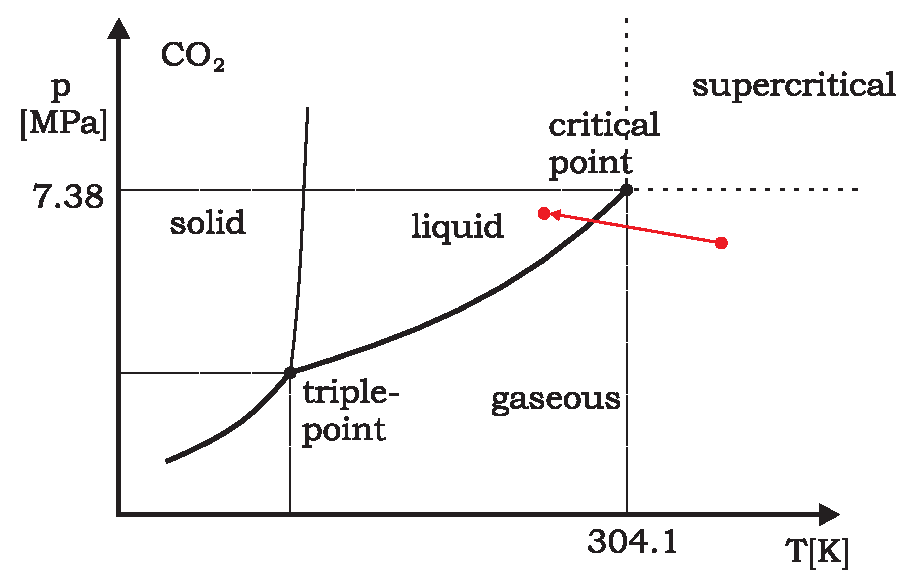
\includegraphics[width=0.9\textwidth]{figures/phase-diagram-co2.eps}
\caption{Phase diagram of carbon dioxide. The two extreme conditions ($\unit[400]{K}$ at $\unit[6.5]{MPa}$ and $\unit[300]{K}$ at $\unit[7]{MPa}$) are crossing a phase boundary of \co2, so a phase change from hot gas to  to liquid state will be forced.}
\label{fig-eos-phase}
\end{figure}

%
\begin{table}[htbp]
\caption{References for fluid properties of \ch4, \co2, \h2o, and \n2}
%\centering
\label{tab-eos-fluid_prop_bm}
\begin{center} 	
\begin{tabular}{llll}
\toprule
\textbf{Fluid} 	& \textbf{Specifier}   & \textbf{Density} 	& \textbf{Viscosity}  \\
\midrule
Methane \ch4			& CH4-RK     			&  \cite{RedKwo:49} & Friend, 1989 \cite{FriElyIng:89}\\
            			& CH4-PR     			&  \cite{PenRob:75} &    \\
             			& CH4-HE    			&  \cite{SetWag:91} &    \\
\midrule
Carbon dioxide \co2 	& CO2-RK     			&  \cite{RedKwo:49}  & Fenghour, 1998 \cite{FenWakVes:98} \\
                    	& CO2-PR     			&  \cite{PenRob:75}  &    \\
                   		& CO2-HE     			&  \cite{SpaWag:96}  &    \\
\midrule
Water \h2o 				& H2O-RK     			&  \cite{RedKwo:49}  & IAPWS, 1998 \cite{IAPWS:08a}      \\ 
           				& H2O-PR     			&  \cite{PenRob:75}  &    \\
           				& H2O-HE     			&  \cite{WagPru:02}  &    \\
\midrule
Nitrogen \n2 			& N2-RK      			& \cite{RedKwo:49}   & Stephan, 1987 \cite{SteKraLae:87} \\
             			& N2-PR     			&  \cite{PenRob:75}  &    \\
             			& N2-HE     			&  \cite{SpaLem:00}  &    \\
\bottomrule
\end{tabular}
\end{center}
\end{table}

%% \newfont{\tensy}{cmsy10}
%% \newcommand{\chemical}[1]{{$\fontdiment16\tensy=3.0pt\fontdiment17\tensy=3.0pt \mathrm{#1}$}}


%\subsection{Thermodynamic properties}

\subsection{Density} \label{eos-density}

In subterranean oil and gas reservoirs, properties of gases and liquids strongly depend from environmental pressure and temperature conditions. Equations of state (EOS) may be used to describe the relationship of volume, pressure and temperature of a real fluid. The knowledge of a fluids volume or its density is essential to estimate further thermodynamic properties. The first EOS for real gases, which was based on the ideal gas law, was presented by Johannes Diderik \textsc{van der Waals} in 1873 \cite{VanWaa:73}. In 1910 he received the Nobel prize for the development of the equation

\begin{equation}
p=\frac{RT}{V_m-b}-\frac{a}{V^2_m}
\label{eq-van-der-waals}
\end{equation}

where $p$ is the pressure, $R$ is the gas constant, $T$ is the temperature, $V_m$ is the molare volume and $a$ and $b$ are correcting parameters. 

%For the development of this equation \eqref{eq-van-der-waals}, \textsc{van der Waals} received the Nobel prize in 1910.
%
%\begin{equation}
%P=\frac{RT}{v-b}-\frac{a}{v^2}
%\label{eq-van-der-waals}
%\end{equation}

%In the current version of GeoSys\,(4.10.0), three different Equations of state are implemented. 
%\begin{itemize}
%	\item \textsc{Redlich-Kwong}, 1949 \cite{RedKwo:49}
%	\item \textsc{Peng-Robinson}, 1975 \cite{PenRob:75}
%	\item Fundamental equations, see \cite{SpaWag:96},\cite{PruWag:95},\cite{BueWag:06},  \cite{SpaLem:00}, and \cite{SetWag:91}
%\end{itemize}

Following three different EOS will be described, which are implemented in version GeoSys\,(4.10.00), based on the \textsc{van der Waals}-equation~\eqref{eq-van-der-waals}. % JG Satzumstellung

\paragraph{Redlich-Kwong equation of state (RKEOS)}
The Equation of \textsc{Redlich} and \textsc{Kwong} from 1949 \eqref{eq-rkeos1} represents just a little improvement of the van der Waals equation \cite{RedKwo:49}. It is given as 														

\begin{equation}
p=\frac{RT}{V_m-b}-\frac{a}{T^{0.5}\,V_m\,(V_m+b)}.
\label{eq-rkeos1}
\end{equation}

Its results are satisfactory only for temperatures above the critical point (see Tab.~\ref{tab-eos2}). 

\begin{table}[H]
  \caption{\label{tab-eos2}Fluid properties used in equations of state, where $\omega$ is the acentric factor, $T_c$ and $p_c$ are temperature und pressure at the critical point and $R$ ist the gas constant.}
  \begin{center}
\begin{tabular}{lrrrr}
\toprule
  substance 		& $\omega$ [-]  & $T_c$ [K] & $p_c$ [MPa] & $R$ [J/kg/K]\\
\midrule
  Carbon dioxide & 0.239  			& 304.13 & 7.38 		& 188.9\\
  Ethane         & 0.099  			& 305.32	& 4.87 		& 276.5\\
  Methane        & 0.011  			& 190.56 & 4.60 		& 518.3\\
  Water          & 0.344  			& 647.10 & 22.06 		& 461.5\\
\bottomrule
\end{tabular}
\end{center}
\end{table}

Equation \eqref{eq-rkeos1} can be recasted as a cubic equation in terms of volume

\begin{equation}
V_m^3-\frac{RT}{p}V_m^2-\left(\frac{RTb}{p}-\frac{a}{T^{0.5}p}+b^2\right)V_m-\frac{ab}{T^{0.5}p}=0.
\label{eq-rkeos2}
\end{equation}
              
This equation yields to one or three real roots depending on the number of phases in the system. In the two-phase region, the largest positive root represents the molar volume of the gas phase while the smallest root correspondes to the volume of the liquid phase. The correcting terms $a$ and $b$ are given as
													
\begin{equation}
a=0.4275\,\frac{R^2 T_c^{2.5}}{p_c}
\label{eq-rkeos_a}
\end{equation}

and

\begin{equation}
b= 0.0866\,\frac{RT_c}{p_c}
\label{eq-rkeos_b}
\end{equation}

where $T_c$ and $p_c$ are Temperature and pressure at the critical point (see Tab.~\ref{tab-eos2}). Figs.~\ref{fig-eos-dens-ch4-co2} and \ref{fig-eos-dens-h2o-n2} show the results of the RKEOS for several substances at four different temperatures in comparison to other equations of state.


%\begin{figure}
%\begin{minipage}{0.49\textwidth}
%\centering
%\includegraphics[width=1\textwidth]{FLUID_PROPERTIES/figures/dens-ch4.eps}
%\caption[bild1]{Density of $\mathrm{CH_4}$ derived by different equations of state}
%\label{fig-eos-dens-ch4}
%\end{minipage}
%%
%\hspace{0.02\textwidth
%}
%\begin{minipage}{0.49\textwidth}
%\centering
%\includegraphics[width=1\textwidth]{FLUID_PROPERTIES/figures/dens-co2.eps}
%\caption[bild2]{Density of $\mathrm{CO_2}$ derived by different equations of state}
%\label{fig-eos-dens-co2}
%\end{minipage}
%\end{figure}


\begin{figure}
\subfigure[]{\label{fig-eos-dens-ch4}\includegraphics[width=0.5\textwidth]{FLUID_PROPERTIES/figures/dens-ch4.eps}}
\hfill
\subfigure[]{\label{fig-eos-dens-co2}\includegraphics[width=0.5\textwidth]{FLUID_PROPERTIES/figures/dens-co2.eps}}
\caption[]{\label{fig-eos-dens-ch4-co2}Density of \ch4~\subref{fig-eos-dens-ch4} and \co2~\subref{fig-eos-dens-co2} derived by different EOS. There stand 
\setlength{\unitlength}{1ex}
\begin{picture}(5,1)
\thicklines \put(0,0.5){\line(1,0){5}}
\end{picture}
for the \textsc{Helmholtz} Free Energy,
\begin{picture}(5,1)
\thicklines \multiput(0,0.5)(2,0){3}{\line(1,0){1}}
\end{picture}
for the PREOS and
\begin{picture}(5,1)
\thicklines \multiput(0,0.5)(2,0){3}{\line(1,0){1}}\multiput(1.4,0.5)(2,0){2}{\line(1,0){0.25}}
\end{picture}
for the RKEOS. The colours refer to different temperatures (\textcolor{blue}{blue} - $\unit[280]{K}$, \textcolor{violet}{violet} - $\unit[320]{K}$, \textcolor{purple}{pink} - $\unit[400]{K}$, \textcolor{red}{red} - $\unit[680]{K}$).}
\end{figure}




%\begin{figure}
%\begin{minipage}{0.49\textwidth}
%\centering
%\includegraphics[width=1\textwidth]{FLUID_PROPERTIES/figures/dens-h2o.eps}
%\caption[bild1]{Density of $\mathrm{H_2O}$ derived by different equations of state}
%\label{fig-eos-dens-h2o}
%\end{minipage}
%%
%\hspace{0.02\textwidth
%}
%\begin{minipage}{0.49\textwidth}
%\centering
%\includegraphics[width=1\textwidth]{FLUID_PROPERTIES/figures/dens-n2.eps}
%\caption[bild2]{Density of $\mathrm{N_2}$ derived by different equations of state}
%\label{fig-eos-dens-n2}
%\end{minipage}
%\end{figure}


\begin{figure}
\subfigure[]{\label{fig-eos-dens-h2o}\includegraphics[width=0.5\textwidth]{FLUID_PROPERTIES/figures/dens-h2o.eps}}
\hfill
\subfigure[]{\label{fig-eos-dens-n2}\includegraphics[width=0.5\textwidth]{FLUID_PROPERTIES/figures/dens-n2.eps}}
\caption[]{\label{fig-eos-dens-h2o-n2}Density of \h2o~\subref{fig-eos-dens-h2o} and \n2~\subref{fig-eos-dens-n2} derived by different EOS. There stand 
\setlength{\unitlength}{1ex}
\begin{picture}(5,1)
\thicklines \put(0,0.5){\line(1,0){5}}
\end{picture}
for the \textsc{Helmholtz} Free Energy,
\begin{picture}(5,1)
\thicklines \multiput(0,0.5)(2,0){3}{\line(1,0){1}}
\end{picture}
for the PREOS and
\begin{picture}(5,1)
\thicklines \multiput(0,0.5)(2,0){3}{\line(1,0){1}}\multiput(1.4,0.5)(2,0){2}{\line(1,0){0.25}}
\end{picture}
for the RKEOS. The colours refer to different temperatures (\textcolor{blue}{blue} - $\unit[280]{K}$, \textcolor{violet}{violet} - $\unit[320]{K}$, \textcolor{purple}{pink} - $\unit[400]{K}$, \textcolor{red}{red} - $\unit[680]{K}$).}
\end{figure}



\paragraph{Peng-Robinson equation of state (PREOS)}
D.\,Y.\,\textsc{Peng} and D.\,B.\,\textsc{Robinson} presented an improvement of the RKEOS in 1975 \cite{PenRob:75}. The proposed equation is also a two-constant van der Waals-Type equation and combines simplicity and accuracy. The PREOS is very simple to solve and gives satisfying results within the whole fluid redion of a gas. It is given in the form

\begin{equation}
p=\frac{RT}{V_m-b}-\frac{a(T_c)\cdot \alpha (T_r,\omega)}{V_m^2+2\cdot bV_m-b^2}
\label{eq-preos1}
\end{equation}

where $a$ and $b$ are correcting terms. They can be derived by %\eqref{eq-preosa} and \eqref{eq-preosb} 

\begin{equation} 
a(T_c) = 0.45724\,\frac{R^2T_{c}^{2}}{p_c}
\label{eq-preosa}
\end{equation}

and

\begin{equation} 
b(T_c) = 0.07780\,\frac{RT_c}{p_c}
\label{eq-preosb}
\end{equation}

for the particular fluids under specification of pressure and temperature at the critical point.
Parameter $\alpha(T_r,\omega)$ is a dimensionless function of reduced temperature $T_r$ and acentric factor $\omega$. It is given as

\begin{equation} 
\alpha = \left( 1+ \left(0.37464 + 1.54226\,\omega - 0.26992\,\omega^2\right)\left(1-T_r^{0.5}\right)\right)^2
\label{eq-preosalpha1}
\end{equation}

for $\omega\leq{0.49}$ and

\begin{equation} 
\alpha = \left( 1+ \left(0.379642 + \left(1.48503-\left(1.164423-1.016666\,\omega\right)\omega\right)\omega\right)\left(1-T_r^{0.5}\right)\right)^2
\label{eq-preosalpha2}
\end{equation}

for $\omega > 0.49$. 

Tab.~\ref{tab-eos2} shows acentric factors and critical parameters for different real gases. The resulting density distribution of the 
PREOS is shown in Figs.~\ref{fig-eos-dens-ch4-co2} and \ref{fig-eos-dens-h2o-n2} at four different temperatures. 

%-----> JG: Vorschlag fr diesen Abschnitt s.u.

%\paragraph {Fundamental equations}				
%For highly precise results it is necessary to adapt fundamental equations based on the free energy, see \eqref{eq-fhe1}. Many authors used this approach to develop EOS for different substances, e.\,g.\,:
%
%\begin{itemize}
%\item \textsc{Span\&Wagner} \cite{SpaWag:96}, \cite{Spa:93}, \cite{SpaLem:00} for carbon dioxide and for nitrogen,
%\item \textsc{Pru\&Wagner} \cite{PruWag:95}, \cite{WagPru:02} for water,
%\item \textsc{Bcker\&Wagner} \cite{BueWag:06} for ethane and
%\item \textsc{Setzmann\&Wagner} \cite{SetWag:91} for methane.
%\end{itemize}
%
%Equation \eqref{eq-fhe1} shows \textsc{Helmholtz} free energy in dependence from density $\rho$ and temperature $T$ in its dimensionless shape, where $\phi^{o}$ is an ideal gas part and $\phi^{r}$ represents a residual part. 
%
%\begin{equation}
%\frac{f(\rho,T)}{RT}=\phi(\delta,\tau)=\phi^{o}(\delta,\tau)+\phi^{r}(\delta,\tau)
%\label{eq-fhe1}
%\end{equation}
%where $\delta=\rho/\rho_c$ and $\tau=T_c/T$\footnote{$\rho_c$ and $T_c$ are density and temperature at the critical point, see table \ref{tab-eos2}}
%The fundamental equation (\ref{eq-fhe1}) according to \textsc{Wagner} et al. (\cite{SpaWag:96},\cite{PruWag:95},\cite{BueWag:06}, and \cite{SetWag:91}) is one of the most precise EOS at present. The Equation and its derivatives can be used to describe all thermodynamic properties of a pure substance depending on density and temperature. So, it is necessary to solve the relationship between density, pressure, and temperature (eq. \ref{eq-fhe-dens}) iteratevly.
%
%\begin{equation}
%\frac{p(\delta,\tau)}{\rho RT}=1+\delta \frac{\partial \phi^r}{\partial \delta}
%\label{eq-fhe-dens}
%\end{equation}
%
%For water, the equation became international standard for the IAPWS since 1995. Certainly, the equation is complicated to solve and requires long computing time. Therefore, in the current version of Geosys, it is possible to choose between an iterative solving algorithm and an interpolation of density values out of a database. 
%


\paragraph {Fundamental equations}			
For highly precise results it is necessary to adapt fundamental equations based on the free energy. The \textsc{Helmholtz} free energy is given as

\begin{equation}
\frac{f(\rho,T)}{RT}=\phi(\delta,\tau)=\phi^{o}(\delta,\tau)+\phi^{r}(\delta,\tau)
\label{eq-fhe1}
\end{equation}
in dependence from density $\rho$ and temperature $T$ in its dimensionless form. These dimensionless parts are given as the terms $\delta=\rho/\rho_c$ and $\tau=T_c/T$, whereas $\rho_c$ and $T_c$ are density and temperature at the critical point (see Tab.~\ref{tab-eos2}).  The \textsc{Helmholtz} free energy provides relations between density, temperature and all thermodynamic properties of a fluid, which are expressed in the parameter $\phi^{o}$ as the ideal gas part and $\phi^{r}$ as the residual part. For their derivatives in the short forms like
$\phi^r_\delta$,\hspace{0.1cm} 
$\phi^r_{\delta\delta}$,\hspace{0.1cm} 
$\phi^r_\tau$,\hspace{0.1cm} 
$\phi^r_{\tau\tau}$,\hspace{0.1cm} 
$\phi^r_{\delta\tau}$,\hspace{0.1cm}
$\phi^o_\tau$,\hspace{0.1cm} 
$\phi^o_{\tau\tau}$
it is refered to \cite{SpaWag:96}.

Many authors used the approach of \textsc{Helmholtz} free energy to develop EOS for different substances, e.\,g.\,:

\begin{itemize}
\item \textsc{Span\&Wagner} \cite{SpaWag:96}, \cite{Spa:93}, \cite{SpaLem:00} for carbon dioxide and for nitrogen,
\item \textsc{Pruß\&Wagner} \cite{PruWag:95}, \cite{WagPru:02} for water,
\item \textsc{Bücker\&Wagner} \cite{BueWag:06} for ethane and
\item \textsc{Setzmann\&Wagner} \cite{SetWag:91} for methane.
\end{itemize}

The fundamental equation (\ref{eq-fhe1}) according to \textsc{Wagner} et al.\ (\cite{SpaWag:96},\cite{PruWag:95},\cite{BueWag:06}, and \cite{SetWag:91}) is one of the most precise EOS at present. The Equation and its derivatives can be used to describe all thermodynamic properties of a pure substance depending on density and temperature. So it is necessary to solve the relationship between density, pressure and temperature  iteratevly, as \eqref{eq-fhe-dens} shows

\begin{equation}
\frac{p(\delta,\tau)}{\rho RT}=1+\delta \frac{\partial \phi^r}{\partial \delta}.
\label{eq-fhe-dens}
\end{equation}

For water, the equation became international standard for the IAPWS\,\footnote{International Association for the Properties of Water and Steam} since 1995. Certainly, the equation is complicated to solve and requires long computing time. Therefore, in the version of GeoSys\,(4.10.00) it is possible to choose between an iterative solving algorithm 
and an interpolation of density values out of a database. 

The semi-empirical fundamental equation \eqref{eq-fhe1} has to be fitted to measurement data by computer algorithms for each substance. Depending on the fluid, there are up to 200 adjusting coefficients to ensure a very accurate fit to the real gas behaviour. For each 
substance, \eqref{eq-fhe1} has separate ranges of validity, which are shown in Tab.~\ref{tab-eos-val}.

\begin{table}[H]
  \caption{\label{tab-eos-val}Ranges of validity of the free \textsc{Helmholtz} equation \eqref{eq-fhe1} for serveral fluids valid from the melting point up to the indicated 
  values.}
 \begin{center}
 \begin{tabular}{lrrl}
  \toprule
  	substance		&$T$ [K]    &$p$ [MPa]	&reference\\
  \midrule
  Carbon dioxide 	& 216 		& 1100 		& \cite{SpaWag:96}, \cite{Spa:93}\\
  Nitrogen      	 & 1000 		& 2200 		& \cite{SpaLem:00}\\
  Ethane        	 & 520 		& 30 			& \cite{BueWag:06}\\ 
  Methane       	 & 625 		& 1000 		& \cite{SetWag:91}\\
  Water         	 & 1273 		& 1000 		& \cite{PruWag:95}, \cite{WagPru:02}\\
 \bottomrule
 \end{tabular}
 \end{center}
\end{table}

% The \textsc{Helmholtz} free energy provides relations between density, temperature and all thermodynamic properties of a fluid. Some of them are shown here: 
%
%$\phi^r_\delta = \left[\frac{\partial\phi^r}{\partial\delta}\right]_\tau$, $\phi^r_\delta\delta = \left[\frac{\partial^2\phi^r}{\partial\delta^2}\right]_\tau$, 
%$\phi^r_\tau = \left[\frac{\partial\phi^r}{\partial\tau}\right]_\delta$, $\phi^r_\tau\tau = \left[\frac{\partial^2\phi^r}{\partial\tau^2}\right]_\delta$, 
%$\phi^r_\delta\tau = \left[\frac{\partial^2\phi^r}{\partial\delta\partial\tau}\right]$, $\phi^o_\tau = \left[\frac{\partial\phi^o}{\partial\tau}\right]_\delta$, 
%$\phi^o_\tau\tau = \left[\frac{\partial^2\phi^o}{\partial\tau^2}\right]_\delta$.

%#####################################################################################################################
\subsection{Enthalpy}

The specific enthalpy $h$ is the whole amount of energy of a fluid. It consists of the internal energy and the volume changing work. It can be expressed by deviations of the free \textsc{Helmholtz} energy as

\begin{equation}
\frac{h(\delta,\tau)}{RT}=1+\tau\left(\phi^o_\tau+\phi^r_\tau\right)+\delta\phi^r_\delta.
\label{eq-fhe-enthalpy}
\end{equation}

%% \begin{figure}
%% \begin{minipage}{0.49\textwidth}
%% \centering
%% \includegraphics[width=1\textwidth]{FLUID_PROPERTIES/figures/enthalpy-co2.eps}
%% \caption[bild1]{Enthalpy of $\mathrm{CO_2}$ based on different equations of state}
%% \label{fig-eos-enthalpy-co2}
%% \end{minipage}
%% %
%% \hspace{0.02\textwidth}
%% %
%% \begin{minipage}{0.49\textwidth}
%% \centering
%% \includegraphics[width=1\textwidth]{FLUID_PROPERTIES/figures/entropy-co2.eps}
%% \caption[bild2]{Entropy of $\mathrm{CO_2}$ based on different equations of state}
%% \label{fig-eos-entropy-co2}
%% \end{minipage}
%% \end{figure}


%#####################################################################################################################
\subsection{Entropy}

The entropy $s$ represents which plenty of the energy of a system is potentially available to do work and which plenty of it is potentially defined as heat. In classical thermodynamics, the validity for the entropy is the thermodynamical system in equilibrium. The following equation is given for the entropy:

\begin{equation}
\frac{s(\delta,\tau)}{R}=\tau\left(\phi^o_\tau+\phi^r_\tau\right)-\phi^o-\phi^r.
\label{eq-fhe-entropy}
\end{equation}
%#####################################################################################################################
\subsection{Heat capacity}

The specific heat capacity of a fluid is defined as the amount of heat which is needed to increase the temperature of a fluid of $\unit[1]{kg}$ by $\unit[1]{K}$. In thermodynamics, it is distinguished between a heat capacity at constant pressure, the isobaric heat capacity, and a heat capacity at constant volume, the isochoric heat capacity. Both can be expressed in terms of free \textsc{Helmholtz} energy, like the following equations show:

\begin{itemize}
\item[]isobaric heat capacity
\end{itemize}
\begin{equation}
\frac{c_p(\delta,\tau)}{R}=-\tau^2\left(\phi^o_{\tau\tau}+\phi^r_{\tau\tau}\right)+\frac{\left(1+\delta\phi^r_\delta-\delta\tau\phi^r_{\delta\tau}\right)^2}{\left(1+2\delta\phi^r_\delta+\delta^2\phi^r_{\delta\delta}\right)} 
\label{eq-fhe-isobar}
\end{equation}

\begin{itemize}
\item[]isochoric heat capacity
\begin{equation}
\frac{c_v(\delta,\tau}{R}=-\tau^2\left(\phi^o_{\tau\tau}+\phi^r_{\tau\tau}\right).
\label{eq-fhe-isochor}
\end{equation}
\end{itemize}

%% \begin{figure}
%% \begin{minipage}{0.49\textwidth}
%% \centering
%% \includegraphics[width=1\textwidth]{FLUID_PROPERTIES/figures/isobar-co2.eps}
%% \caption[bild1]{Isobaric heat capacity of $\mathrm{CO_2}$ based on different equations of state}
%% \label{fig-eos-isobar-co2}
%% \end{minipage}
%% %
%% \hspace{0.02\textwidth}
%% %
%% \begin{minipage}{0.49\textwidth}
%% \centering
%% \includegraphics[width=1\textwidth]{FLUID_PROPERTIES/figures/isochor-co2.eps}
%% \caption[bild2]{Isochoric heat capacity of $\mathrm{CO_2}$ based on different equations of state}
%% \label{fig-eos-isochor-co2}
%% \end{minipage}
%% \end{figure}




%\begin{figure}%[ht]
%\begin{minipage}{0.49\textwidth}
%\centering
%\includegraphics[width=1\textwidth]{FLUID_PROPERTIES/figures/enthalpy-co2.eps}
%\caption[bild1]{Enthalpy of $\mathrm{CO_2}$ based on different equations of state}
%\label{fig-eos-enthalpy-co2}
%\end{minipage}
%%
%\hspace{0.02\textwidth}
%%
%\begin{minipage}{0.49\textwidth}
%\centering
%\includegraphics[width=1\textwidth]{FLUID_PROPERTIES/figures/entropy-co2.eps}
%\caption[bild2]{Entropy of $\mathrm{CO_2}$ based on different equations of state}
%\label{fig-eos-entropy-co2}
%\end{minipage}
%
%\vspace{2,5cm}
%%% \end{figure}
%%% 
%%% \begin{figure}[h]
%\begin{minipage}{0.49\textwidth}
%\centering
%\includegraphics[width=1\textwidth]{FLUID_PROPERTIES/figures/isobar-co2.eps}
%\caption[bild1]{Isobaric heat capacity of $\mathrm{CO_2}$ based on different equations of state}
%\label{fig-eos-isobar-co2}
%\end{minipage}
%%
%\hspace{0.02\textwidth}
%%
%\begin{minipage}{0.49\textwidth}
%\centering
%\includegraphics[width=1\textwidth]{FLUID_PROPERTIES/figures/isochor-co2.eps}
%\caption[bild2]{Isochoric heat capacity of $\mathrm{CO_2}$ based on different equations of state}
%\label{fig-eos-isochor-co2}
%\end{minipage}
%\end{figure}


\begin{figure}[t]
\subfigure[]{\label{fig-eos-enthalpy-co2}\includegraphics[width=0.5\textwidth]{FLUID_PROPERTIES/figures/enthalpy-co2.eps}}
\hfill
\subfigure[]{\label{fig-eos-entropy-co2}\includegraphics[width=0.5\textwidth]{FLUID_PROPERTIES/figures/entropy-co2.eps}}
\caption[]{\label{fig-eos-enthalpy-entropy-co2}Enthalpy~\subref{fig-eos-enthalpy-co2} and entropy~\subref{fig-eos-entropy-co2} of $\mathrm{CO_2}$ based on different EOS. There stand 
\setlength{\unitlength}{1ex}
\begin{picture}(5,1)
\thicklines \put(0,0.5){\line(1,0){5}}
\end{picture}
for the \textsc{Helmholtz} Free Energy,
\begin{picture}(5,1)
\thicklines \multiput(0,0.5)(2,0){3}{\line(1,0){1}}
\end{picture}
for the PREOS and
\begin{picture}(5,1)
\thicklines \multiput(0,0.5)(2,0){3}{\line(1,0){1}}\multiput(1.4,0.5)(2,0){2}{\line(1,0){0.25}}
\end{picture}
for the RKEOS. The colours refer to different temperatures (\textcolor{blue}{blue} - $\unit[280]{K}$, \textcolor{violet}{violet} - $\unit[320]{K}$, \textcolor{purple}{pink} - $\unit[400]{K}$, \textcolor{red}{red} - $\unit[680]{K}$).}
\end{figure}

\begin{figure}[h]
\subfigure[]{\label{fig-eos-isobar-co2}\includegraphics[width=0.5\textwidth]{FLUID_PROPERTIES/figures/isobar-co2.eps}}
\hfill
\subfigure[]{\label{fig-eos-isochor-co2}\includegraphics[width=0.5\textwidth]{FLUID_PROPERTIES/figures/isochor-co2.eps}}
\caption[]{\label{fig-eos-isobar-isochor-co2}Isobaric heat capacity~\subref{fig-eos-isobar-co2} and isochoric heat capacity~\subref{fig-eos-isochor-co2} of $\mathrm{CO_2}$ based on different EOS. There stand 
\setlength{\unitlength}{1ex}
\begin{picture}(5,1)
\thicklines \put(0,0.5){\line(1,0){5}}
\end{picture}
for the \textsc{Helmholtz} Free Energy,
\begin{picture}(5,1)
\thicklines \multiput(0,0.5)(2,0){3}{\line(1,0){1}}
\end{picture}
for the PREOS and
\begin{picture}(5,1)
\thicklines \multiput(0,0.5)(2,0){3}{\line(1,0){1}}\multiput(1.4,0.5)(2,0){2}{\line(1,0){0.25}}
\end{picture}
for the RKEOS. The colours refer to different temperatures (\textcolor{blue}{blue} - $\unit[280]{K}$, \textcolor{violet}{violet} - $\unit[320]{K}$, \textcolor{purple}{pink} - $\unit[400]{K}$, \textcolor{red}{red} - $\unit[680]{K}$).}
\end{figure}




Due to the high number of adjusting coefficients, the properties based on the \textsc{Helmholtz} free energy may be seen as very 
accurate. On the other hand, the iterative solution of \eqref{eq-fhe-dens} takes long computing times, so for long-term simulations or for simulations with a high number of elements, it would be better to use the \textsc{van der Waals}-type equations of \textsc{Redlich-Kwong} or \textsc{Peng-Robinson}. These cubic equations are easy to solve and lead to results very fast. Figs.~\ref{fig-eos-enthalpy-entropy-co2} and \ref{fig-eos-isobar-isochor-co2} illustrate, in which range of temperature and pressure those simple EOS may be used. Here, thermodynamical properties of carbon dioxide based on temperature and density are shown calculated by different EOS. In general, if temperature rises while pressure is declining, the behaviour of a fluid approaches to that of the ideal gas and the cubic equations of state give suitable results. For instance, the resulting entropy and enthalpy values of carbon dioxide at low pressures and high temperatures are identical, regardless of the density model they are based on (see Fig.~\ref{fig-eos-enthalpy-co2} and \ref{fig-eos-entropy-co2}). In the liquid and the dense supercritical region, the results based on different EOS diverge increasingly.


%% \begin{figure}[t]
%% \begin{minipage}{0.49\textwidth}
%% \centering
%% \includegraphics[width=1\textwidth]{FLUID_PROPERTIES/figures/enthalpy-co2.eps}
%% \caption[bild1]{Enthalpy of $\mathrm{CO_2}$ based on different equations of state}
%% \label{fig-eos-enthalpy-co2}
%% \end{minipage}
%% \hspace{0.02\textwidth}
%% \begin{minipage}{0.49\textwidth}
%% \centering
%% \includegraphics[width=1\textwidth]{FLUID_PROPERTIES/figures/entropy-co2.eps}
%% \caption[bild2]{Entropy of $\mathrm{CO_2}$ based on different equations of state}
%% \label{fig-eos-entropy-co2}
%% \end{minipage}
%% %\end{figure}
%% %\begin{figure}[h]
%% \begin{minipage}{0.49\textwidth}
%% \centering
%% \includegraphics[width=1\textwidth]{FLUID_PROPERTIES/figures/isobar-co2.eps}
%% \caption[bild1]{Isobaric heat capacity of $\mathrm{CO_2}$ based on different equations of state}
%% \label{fig-eos-isobar-co2}
%% \end{minipage}
%% \hspace{0.02\textwidth}
%% \begin{minipage}{0.49\textwidth}
%% \centering
%% \includegraphics[width=1\textwidth]{FLUID_PROPERTIES/figures/isochor-co2.eps}
%% \caption[bild2]{Isochoric heat capacity of $\mathrm{CO_2}$ based on different equations of state}
%% \label{fig-eos-isochor-co2}
%% \end{minipage}
%% \end{figure}


In addition, in the vicinity of the saturation curve, the results based on the \textsc{van der Waals}-type EOS may show large variations compared to the fundamental equation based curves (\textsc{Helmholtz} free energy). Particularly, this becomes apparent from Figs.~\ref{fig-eos-isobar-co2} and \ref{fig-eos-isochor-co2}, where the heat capacities of $\mathrm{CO_2}$ are given. The heat capacities at $\unit[400]{K}$ and $\unit[680]{K}$ (in the supercritical region of $\mathrm{CO_2}$, where no phase boundary exists) are identical, independent from according density model. Within the two-phase region at $\unit[280]{K}$ and $\unit[320]{K}$, a strong deviation at the phase boundary can be seen.

For water, the cubic EOS are not suitable. Water is a high critical fluid, so its properties are to complex to be described by simple approaches. As we can see in Fig.~\ref{fig-eos-dens-h2o}, the RKEOS, as well as the PREOS equation give viable results only at pressures below $\unit[1]{MPa}$ and at high temperatures. Therefor it is recommended to use the fundamental equation of the \textsc{Helmholtz} free energy to estimate the density of water. 


       
%#####################################################################################################################			
%\subsection{Transport properties}
%\label{sec_TP}
%############################################################################################################################
\subsection {Viscosity} \label{sec-viscosity}
Many authors developed correlation equations for viscosity $\eta$ of fluids at a density $\rho$ and a temperature $T$. Those correlation equations may be composed of two or three terms, like

\begin{equation}
\eta (\rho,T) = \eta_{0} (T) + \eta_{ex} (\rho,T)
	\label{eq-two-term-visc}
\end{equation}

or

\begin{equation}
\eta (\rho,T) = \eta_{0} (T) + \Delta \eta (\rho,T) + \Delta \eta_c (\rho,T).
	\label{eq-three-term-visc}
\end{equation}


In the two-term form, the viscosity correlation consists of a zero-density limit viscosity $\eta_0(T)$ at a temperature $T$, and an excess contribution viscosity $\eta_{ex}(\rho,T)$ at a density $\rho$ and a temperature $T$. This type of correlation function is used (among others) by \textsc{Friend} et al.\ \cite{FriElyIng:89} or \textsc{Stephan} et al.\ \cite{SteKraLae:87}. The formulation can be enhaced by a term describing the viscosity in the immediate vicinity of the critical point, $\Delta \eta (\rho,T)$ \eqref{eq-three-term-visc}, as described in \textsc{Fenghour} et al.\ \cite{FenWakVes:98} or \textsc{Huber} et al.\ \cite{IAPWS:08a}. An overview about the used viscosity correlations for several substances is given in Tab.~\ref{tab-eos-visc}. To show an example, Fig.~\ref{fig-eos-visc-co2} portrays the resulting viscosities for carbon dioxide based on densities of different EOS.


\begin{table}[H]
  \caption{\label{tab-eos-visc}Ranges of $T$ and $p$ validity for viscosity correlations for several substances.}
  \begin{center}
  \begin{tabular}{lrrl}
  \toprule
  substance 		& $T$ [K]		& $p$ [MPa] 	& reference \\
  \midrule
  Carbon dioxide 	& 200--1500		& $\leq{300}$ 	& \cite{FenWakVes:98}\\
  Nitrogen       	& 70--1100		& $\leq{100}$ 	& \cite{SteKraLae:87}\\  
  Ethane         	& 90--625		& $\leq{30}$ 	& \cite{FriIngEly:91}\\ 
  Methane       	&	91--600		& $\leq{100}$	& \cite{FriElyIng:89}\\  
  Water          	& 273--1173		& $\leq{100}$	& \cite{IAPWS:08a}\\
  \bottomrule
 \end{tabular}
 \end{center}
\end{table}
  


%############################################################################################################################
\subsection {Thermal conductivity} \label{sec-thermal-conductivity}
%$~~$ \\
Similar to the correlations between viscosity and $T$ and $p$, the thermal conductivity $\lambda$ can be expressed by an equation consisting of the following three parts (see \cite{VesWak:90}): A conductivity in the limit of zero-density $\lambda^0(0,T)$, where only two-body interaction occurs, a term $\Delta_c\lambda (\rho,T)$ wich enhances the property function in the critical region of the fluid, and finally $\Delta\lambda (\rho,T)$ which represents the contribution of all other effects to the thermal conductivity at elevated densities including many-body collisions, molecular-velocity correlations and collisional transfer. This equation is

\begin{equation}
\lambda (\rho,T) = \lambda^0 (T) + \Delta\lambda (\rho)+ \Delta_c \lambda (\rho,T).
\label{EqEOS_visc}
\end{equation}

Fig.~\ref{fig-eos-hc-co2} shows the thermal conductivity of carbon dioxide at four temperatures based on different EOS. In Tab.~\ref{tab-eos-hc} the ranges for the validity of $T$ and $p$ concerning thermal conductivity correlations for several substances are shown.

\begin{table}[H]
 \caption{\label{tab-eos-hc}Ranges of $T$ and $p$ validity for thermal conductivity correlations for several substances.}
 \begin{center}
  \begin{tabular}{lrrl}
 \toprule
   substance 		& $T$ [K] 		& $p$ [MPa] 			& Reference \\
  \midrule
  Carbon dioxide 	& 200--1000		& $\leq{100}$ 			& \cite{FenWakVes:98}\\
  Nitrogen       	& 70--1100		& $\leq{100}$		 	& \cite{SteKraLae:87}\\  
  Ethane         	& $\leq{600}$	& $\leq{70}$		 	& \cite{YouEly:87}\\ 
  Methane       	& $\leq{200}$ 	& $\leq{600}$		 	& \cite{YouEly:87}\\  
  Water          	& $\leq{800}$ 	& $\leq{100}$		 	& \cite{IAPWS:08b}\\
  \bottomrule
 \end{tabular}
 \end{center}
\end{table}

%\begin{figure}
%\begin{minipage}{0.49\textwidth}
%\centering
%\includegraphics[width=1\textwidth]{FLUID_PROPERTIES/figures/viscosity-co2.eps}
%\caption[bild1]{Viscosity of $\mathrm{CO_2}$ based on different EOS}
%\label{fig-eos-visc-co2}
%\end{minipage}
%%
%\hspace{0.02\textwidth
%}
%\begin{minipage}{0.49\textwidth}
%\centering
%\includegraphics[width=1\textwidth]{FLUID_PROPERTIES/figures/heat-conductivity-co2.eps}
%\caption[bild2]{Thermal conductivity of $\mathrm{CO_2}$ based on different EOS}
%\label{fig-eos-hc-co2}
%\end{minipage}
%\end{figure}



\begin{figure}[t]
\subfigure[]{\label{fig-eos-visc-co2}\includegraphics[width=0.5\textwidth]{FLUID_PROPERTIES/figures/viscosity-co2.eps}}
\hfill
\subfigure[]{\label{fig-eos-hc-co2}\includegraphics[width=0.5\textwidth]{FLUID_PROPERTIES/figures/heat-conductivity-co2.eps}}
\caption[]{\label{fig-eos-visc-hc-co2}Viscosity~\subref{fig-eos-visc-co2} and thermal conductivity~\subref{fig-eos-hc-co2} of $\mathrm{CO_2}$ based on different EOS. There stand 
\setlength{\unitlength}{1ex}
\begin{picture}(5,1)
\thicklines \put(0,0.5){\line(1,0){5}}
\end{picture}
for the \textsc{Helmholtz} Free Energy,
\begin{picture}(5,1)
\thicklines \multiput(0,0.5)(2,0){3}{\line(1,0){1}}
\end{picture}
for the PREOS and
\begin{picture}(5,1)
\thicklines \multiput(0,0.5)(2,0){3}{\line(1,0){1}}\multiput(1.4,0.5)(2,0){2}{\line(1,0){0.25}}
\end{picture}
for the RKEOS. The colours refer to different temperatures (\textcolor{blue}{blue} - $\unit[280]{K}$, \textcolor{violet}{violet} - $\unit[320]{K}$, \textcolor{purple}{pink} - $\unit[400]{K}$, \textcolor{red}{red} - $\unit[680]{K}$).}
\end{figure}



%-------------------------------------------------------------------------
\newpage
\section{Mechanical properties}
\label{sec:m_properties}
%\section{Mechanical properties}
%\label{sec:m_properties}

Constitutive equations (i.e. constitutive relations, material laws) are relations between measures of deformation (e.g. strain tensor) and internal force density functions (stress tensor) resulting from the action of external forces. Usually, they are not laws of nature but represent mathematical models intended to characterize the typical material behavior based on physically reasonable assumptions (particularly consistent with the thermodynamic balance relations) and mathematically correct approaches.

\subsection{Effective stress principle}
\label{sec:effstress}

Following the statements given in section~\ref{sec:momentum_balance} the total Cauchy's stress tensor in porous media is decomposed in partial stresses referring to the participating phases (note the sign convention of positive fluid phase pressure $p^{\gamma}$, but negative compressive normal stress for the solid phase).
\begin{equation}
\miu{\sigma}{}{}\,=\,(1-n)\,\mio{\sigma}{s}{}\,-\,n
\left(\sum\limits_{\gamma}S^{\gamma}\,p^{\gamma}\right)\mathbf{I}
\label{eq:totalstress}
\end{equation}
Considering the effective stress principle, relation (\ref{eq:totalstress}) can be modified defining the effective solid stress $\mib{\sigma}{eff}{s}{}$ as well as the overall fluid pressure $p^{\gamma}$
\begin{eqnarray}
\miu{\sigma}{}{} & = & 
(1-n)\left[
\mio{\sigma}{s}{}\,+\,\left(\sum\limits_{\gamma}S^{\gamma}\,p^{\gamma}\right)\mathbf{I}
\right]
\,-\,\left(\sum\limits_{\gamma}S^{\gamma}\,p^{\gamma}\right)\mathbf{I} \nonumber \\
 & = &
\miu{\sigma}{\mathrm{eff}}{}{}
\,-\,\left(\sum\limits_{\gamma}S^{\gamma}\,p^{\gamma}\right)\mathbf{I}
\label{eq:effect_stress}
\end{eqnarray}
The effective solid stress is the total solid stress reduced by the excess pore liquid pressure, but referred to the domain of the overall porous medium. Consequently, its absolute value is lower than the intrinsic stress of the solid skeleton. Constitutive relations for the solid phase of porous media combine the solid skeleton deformation (in terms of the strain tensor) with the effective solid stress. Selected models are presented in the next paragraphs. As they are equally valid for single-phase solid materials as well as for the solid phase of porous media, the special notation of the effective stress tensor will be omitted without loss of generality.

Based on the stress decomposition (\ref{eq:effect_stress}), the equilibrium condition for the porous medium becomes
\begin{equation}
\rho \mio{g}{}{}
+
\,\nabla\,\cdot\,\miu{\sigma}{\mathrm{eff}}{}{}\,
-
\left(\sum\limits_{\gamma}S^{\gamma}\,p^{\gamma}\right)\mathbf{I}
=
\,\mathbf{0}
\label{eq:equi_mod}
\end{equation}

%---
\subsection{Material classes}
\label{sec:matclass}

Usually laboratory tests are performed on specimens to investigate the mechanical behavior. Within this context, similar stress-strain curves can be caused by different physical effects, e.g. a nonlinear stress-strain curve does not necessarily suggest inelastic material behavior. For the sake of clarity, it is possible to introduce a classification of materials based on some essential distinctly identifiable material phenomena. For instance, comparatively simple experiments can be performed to investigate if the stress-strain curves are rate-dependent, and if hysteresis phenomena occur indicating dissipative effects.

\begin{figure}[htb!]
\begin{center}
\footnotesize
\includegraphics[width=0.95\textwidth]{figures/matbehav_el_elpl.eps}
\caption{Experimentally observed rate-independent solid material behavior. Cyclic uniaxial stress-strain curves \cite{Haupt:2002}: elasticity (left) and elastoplasticity (right)}
\label{fig:matbehav_el_elpl}
\end{center}
\end{figure}
\begin{figure}[htb!]
\begin{center}
\footnotesize
\includegraphics[width=0.95\textwidth]{figures/matbehav_vel_vpl.eps}
\caption{Experimentally observed rate-dependent solid material behavior. Cyclic uniaxial stress-strain curves \cite{Haupt:2002}: viscoelasticity (left) and viscoplasticity (right)}
\label{fig:matbehav_vel_vpl}
\end{center}
\end{figure}

\newpage

Based on these assumptions the observable material behavior can be divided into four different basic classes:
\begin{itemize}
\item rate-independent without hysteresis,
\item rate-independent with hysteresis,
\item rate-dependent without hysteresis, and
\item rate-dependent with hysteresis.
\end{itemize}
Figs.~\ref{fig:matbehav_el_elpl} and \ref{fig:matbehav_vel_vpl} schematically show typical cyclic stress-strain curves for these material classes. The equlibrium curves, presented in Figs.~\ref{fig:matbehav_vel_vpl} can be observed as a result of relaxation experiments.

According to the experimental observations, there are four classes of mathematical models matching the material classes defined above:
\begin{itemize}
\item the theory of elasticity describes rate-independent material behavior without hysteresis,
\item the theory of (elasto)plasticity describes rate-independent material behavior with hysteresis,
\item the theory of viscoelasticity describes rate-dependent material behavior without hysteresis, and
\item the theory of viscoplasticity describes rate-dependent material behavior with hysteresis.
\end{itemize}

Physically significant constitutive relations in the uniaxial case can be defined for the four classes of material theories based on so-called rheological models. These complex models consist of a simple networks of individual rheological elements (cf. Fig.~\ref{fig:rheomod_elem}), like
\begin{itemize}
\item elastic springs, which correspond to the linear stress-strain relation
\begin{equation}
\sigma\,=\,k\,\varepsilon
\end{equation}
with the spring constant $k$ representing the proportionality factor,  
\item viscous dashpots, which represent Newtonian viscous substances, and obey a linear relation between stress and strain rate
\begin{equation}
\sigma\,=\,\eta\,\mathop{\varepsilon}\limits^{\miu{.}{}{}}
\end{equation}
with the proportionality factor $\eta$ characterizing the viscosity, and
\item Coulomb friction elements, resisiting any motion until a threshold stress $\sigma^{\star}$ is reached, whereas behind the threshold irreversible deformations occur
\begin{equation}
\varepsilon\,=\,
\left\{
\begin{array}{ll}
0,              & \qquad\mbox{if}\quad\sigma\,<\,\sigma^{\star}  \\[1.5ex]
\varepsilon(t), & \qquad\mbox{if}\quad\sigma\,\geq\,\sigma^{\star}
\end{array}
\right.
\end{equation}
\end{itemize}

\newpage

\begin{figure}[htb!]
\begin{center}
\footnotesize
\includegraphics[width=0.95\textwidth]{figures/rheomod_elements.eps}
\caption{Mathematical modeling of solid material behavior. Basic individual elements of rheological models \cite{JCZ:2007}: spring element (left), dashpot element (middle) and frictional element (right)}
\label{fig:rheomod_elem}
\end{center}
\end{figure}

Differential equations, which are defined based on an appropriate composition of rheological models are only in a few special cases suitable to describe material response to external loading observed in reality. They can rather serve for marking the physical significance of mathematical models within the context of material theories. In Figs.~\ref{fig:rheomod_el_elpl} and \ref{fig:rheomod_vel_vpl} typical rheological models are presented, which characterize the material behavior of the four material classes defined above.

\begin{figure}[htb!]
\begin{center}
\footnotesize
\includegraphics[width=0.95\textwidth]{figures/rheomod_el_elpl.eps}
\caption{Mathematical modeling of rate-independent solid material behavior. Cyclic uniaxial stress-strain curves \cite{Haupt:2002}: elasticity (spring element -- left) and elastoplasticity (spring and frictional elements -- right)}
\label{fig:rheomod_el_elpl}
\end{center}
\end{figure}

\begin{figure}[htb!]
\begin{center}
\footnotesize
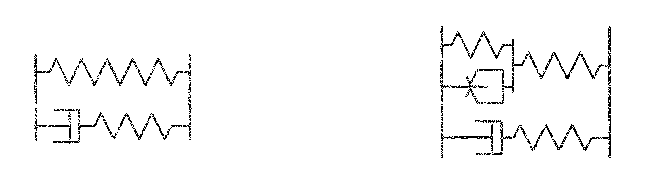
\includegraphics[width=0.95\textwidth]{figures/rheomod_vel_vpl.eps}
\caption{Mathematical modeling of rate-dependent solid material behavior. Cyclic uniaxial stress-strain curves \cite{Haupt:2002}: viscoelasticity (spring and dashpot elements -- left) and viscoplasticity (spring, dashpot, and frictional elements -- right)}
\label{fig:rheomod_vel_vpl}
\end{center}
\end{figure}

In Tab.~\ref{tab:matclass} some typical technical as well as natural (including geological) materials are assigned to the generalized material classes considering their material behavior, which can be observed for characteristic application cases. Generally, the classification of the material behavior depends on the real loading regime (e.g. small or large strains), environmental conditions (e.g. temperature), and the time scale of the physical processes under consideration. Changing one or more of these conditions one and the same material can demonstrate different mechanical behavior. Basically, no materials are actually purely elastic over a wide range of stresses, temperature, and time. Otherwise, developing and using complex constitutive models, which include all observable phenomena is not advisable for practical reasons. Constitutive relations, rather, should represent idealized and simplified models according to the most dominating conditions appearing in the practical applications under consideration.

\renewcommand{\arraystretch}{1.25}
\begin{table}[htb!]
\caption{Generalized classes of solid material behavior, and selected, typical representatives}
\label{tab:matclass}
\begin{center}
%\begin{tabular}{|l||l|l|}
\begin{tabular}{|p{0.18\textwidth}||p{0.37\textwidth}|p{0.33\textwidth}|}
\hline
Material class & Technical/natural material & Geomaterial \\
\hline\hline
elasticity & metals at small strains, & igneous rocks                 \\
           & ceramics,                & (e.g. granite),               \\
           & bone,                    & hard sedimentary rocks        \\
           & most other materials at small strains & (e.g. sandstone) \\
\hline
elastoplasticity & metals at large strains & most soils,                        \\
                 &                         & soft sedimentary rocks (e.g. tuff) \\
\hline
viscoelasticity & rubber,                 & rock salt (halite) \\
                & glass,                  &                    \\
                & soft biological tissues &                    \\
\hline
viscoplasticity & polymers (plastics),       & clay soils, \\
                & wood,                      & clay stone  \\
                & bitumen,                   &             \\
                & metals at high temperature &             \\
\hline
\end{tabular}
\end{center}
\end{table}
\renewcommand{\arraystretch}{1.00}
%
\hfill
%-------------------------------------------------------------------------
\newpage
\subsection{Elasticity}
\label{sec:elasticity}

In a micromechanical point of view, elasticity is predominantly caused by the evolution of interatomic forces in response to the impact of
external forces. It can be observed for crystalline substances (where the atoms are established in regular structures) as well as for
amorphous materials (where the atoms compose irregular structures), and is characterized by reversibility of the deformation processes and
the absence of any hysteresis. Furthermore, it is assumed that the current stress state is uniquely defined by the current strain state,
and does not depend on the strain history. Consequently, within the context of the constitutive model, the stress tensor is a function of
the strain tensor, but it does not depend on the strain rate. 

The isothermal isotropic linear elastic material model 
\begin{equation}
\miu{\sigma}{}{}\,=\,2\mu\,\miu{\varepsilon}{}{}\,+\,\lambda\,\mathrm{tr}(\miu{\varepsilon}{}{})\,\mathbf{I}
\label{eq:hooke_isotherm}
\end{equation}
known as generalized Hooke's law is the simplest of all constititive models for solid material behavior. Instead of the so-called
Lam{\'{e}} constants $\mu$ and $\lambda$, Hooke's law is often represented in terms of other material parameters like the Young's modulus
(i.e. elastic modulus, coefficient of elasticity, modulus of elasticity et al.) $E$, the Poisson's ratio $\nu$, the shear modulus $G$, and
the bulk modulus $K$. Some useful relations between these parameters are as follows:
\begin{eqnarray*}
E & = & \mu\,\ttfrac{2\mu+3\lambda}{\mu+\lambda},\qquad
\nu\,=\,\ttfrac{\lambda}{2(\mu+\lambda)} \\[2.0ex]
\mu & = & \ttfrac{E}{2(1+\nu)},\qquad
\lambda\,=\,\ttfrac{\nu E}{(1+\nu)(1-2\nu)} \\[2.0ex]
G & = & \ttfrac{E}{2(1+\nu)}\,=\,\mu \\[2.0ex]
K & = & \ttfrac{E}{3(1-2\nu)}\,=\,\ttfrac{(\mu+\lambda)(2\mu+3\lambda)}{3}
\end{eqnarray*}
Thus, the coefficients of the consistent material matrix $d\miu{\sigma}{}{}/d\miu{\varepsilon}{}{}$, which is required for the numerical
simulation of mechanical material behavior can be representeed in case of linear elasticity straightforward.
\begin{equation}
\fourtens{C}
\equiv
{C}_{ijkl}\,=\,\frac{d\sigma_{ij}}{d\varepsilon_{kl}}\,=\,2\mu\,\delta_{ik}\,\delta_{jl}\,+\,\lambda\,\delta_{ij}\,\delta_{kl}
\end{equation}

If a coupling of mechanical and thermal processes occur (non-isothermal mechanical processes), in addition to the strain caused by the
impact of external forces a volumetric thermal strain can be observed, which usually is linearly related to
the temperature difference.
\begin{equation}
\miu{\varepsilon}{\mathrm{th}}{}\,=\,\alpha_T\,(T-T_0)\,\mathbf{I}
\end{equation}
Here, $\alpha_T$ denotes the linear thermal expansion coefficient, and $T_0$ the initial temperature. In small strain solid mechanics it is
common practice to consider additive decompositions of the overall strain tensor into several constitutive parts according to the observed
physical phenomena. Considering thermoelastic material behavior, the overall strain tensor consists of an elastic part and a thermal part.
\begin{equation}
\miu{\varepsilon}{}{}\,=\,\miu{\varepsilon}{\mathrm{el}}{}\,+\,\miu{\varepsilon}{\mathrm{th}}{}
\end{equation}
As Hooke's law (\ref{eq:hooke_isotherm}) has to be perceived as a constitutive model, which assigns the local stress state to local elastic
strains, a non-isothermal generalization can be defined easily. 
\begin{equation}
\miu{\sigma}{}{}\,=\,2\mu\,\miu{\varepsilon}{\mathrm{el}}{}\,+\,\lambda\,\mathrm{tr}(\miu{\varepsilon}{\mathrm{el}}{})\,\mathbf{I}
                \,=\,2\mu\,\miu{\varepsilon}{}{}\,+\,\lambda\,\mathrm{tr}(\miu{\varepsilon}{}{})\,\mathbf{I}
                \,-\,(2\mu+3\lambda)\,\miu{\varepsilon}{\mathrm{th}}{}
\label{eq:hooke_nonisotherm}
\end{equation}
A conclusion drawn from Hooke's law of linear elasticity is the specific representation of the equilibrium condition for a thermo-poro-elastic porous medium in case of small strains.
\begin{equation}
\nabla\,\cdot\,
\left(
\miu{\sigma}{\mathrm{eff}}{}{}(\miu{\varepsilon}{}{})\,-\,
\left(\sum\limits_{\gamma}S^{\gamma}\,p^{\gamma}\right)\mathbf{I}\,-\,
\frac{2\mu+3\lambda}{3}\,\alpha_T\,(T-T_0)\,\mathbf{I}
\right)
\,=\,\rho\,\mio{g}{}{}
\label{eq:equi_thermo_poro_elast}
\end{equation}

Although no materials are actually linearly elastic over a wide range of stresses, elastic constitutive models are often quite useful and
accurate in many practical applications, e.g. in rock mechanics. The elastic material parameters given in Tab.~\ref{tab:rockelastpar} for 
selected soils and rocks show the large variation of material parameters, which is typical for geomaterials. 

\renewcommand{\arraystretch}{1.25}
\begin{table}[htb!]
\caption{Elastic material parameters for selected geomaterials}
\label{tab:rockelastpar}
\begin{center}
%\begin{tabular}{|l||l|l|}
\begin{tabular}{|p{0.25\textwidth}||p{0.22\textwidth}|p{0.2\textwidth}|}
\hline
Material & Young's modulus [GPa] & Poisson's ratio \\
\hline\hline
Sand       & 0.03\dots 0.6 & 0.10\dots 0.40 \\
\hline
Clay       & 0.03\dots 0.3 & 0.12\dots 0.40\\
\hline\hline
Clay stone & \ \,3\dots 11   & 0.10\dots 0.27 \\
\hline
Salt rock  & 12\dots 42  & 0.09\dots 0.49 \\
\hline
Sandstone  & \ \,4\dots 19   & 0.12\dots 0.20 \\
\hline
Granite    & 17\dots 56  & 0.11\dots 0.27 \\
\hline
Basalt     & 31\dots 97  & 0.19\dots 0.30 \\
\hline
Limestone  & 13\dots 53  & 0.11\dots 0.40 \\
\hline
\end{tabular}
\end{center}
\end{table}
\renewcommand{\arraystretch}{1.00}

\subsection{Elastoplasticity}
\label{sec:elastoplast}

The phenomenon of plastic yielding can be mainly observed in crystalline solid materials. It is associated with the motion of defects
(so-called dislocations, discontinuities) of the regular atomic structure during deformation. Elastoplastic material behavior is
characterized by elastic material response at the beginning of the deformation process. If a critical stress (the so-called yield stress)
is reached, plastic flow occurs, whereas elastic material behavior can be observed again at the beginning of each unloading phase of a
cyclic loading process.

In case of elastic-perfectly plastic material behavior, the stresses remain unchanged during plastic flow keeping the yield stress value.
Usually, real materials show elastoplastic material behavior with hardening effects, which are distinguished by an increase of stresses
during plastic flow with much lower slope of the stress-strain curve compared to the elastic phases of the entire deformation process.
Elastoplastic material behavior with neglegible elastic share is called rigid plasticity (see Fig.~\ref{fig:plastcases}).

\begin{figure}[htb!]
\begin{center}
\footnotesize
\includegraphics[width=0.95\textwidth]{figures/plastcases.eps}
\caption{Schematic representation of material behavior exhibiting plastic yielding \cite{JCZ:2007}: elastic-plastic with
strain hardening (left), elastic-perfectly plastic (middle), and rigid-perfectly plastic (right)}
\label{fig:plastcases}
\end{center}
\end{figure}

During plastic flow a certain fraction of the strain energy is transformed into thermal energy or stored as internal energy due to a
remodeling of the microstructure. Therefore, analyzing cyclic elastoplastic processes rate-independent hystereses can be observed.
Additionally, plastic deformation processes prove themselves to be irreversible.

In terms of the mathematical modeling of elastoplasticity no explicit stress-strain relation can be defined (no biunique relationship
between these quantities exists) due to the hysteresis effects. Instead, a mathematically ascertainable functional relation can be created
between the stress rate and the elastic strain rate.
\begin{equation}
\miu{\sigma}{}{\dot}\,=\,\fourtens{C}\,\miu{\varepsilon}{\mathrm{el}}{\dot}
\label{eq:elplastmatlaw}
\end{equation}

As shown in the case of thermoelasticity, the overall strain tensor can be additively split into two constitutive parts: an elastic one
$\miu{\varepsilon}{\mathrm{el}}{}$ and the partial plastic strain tensor $\miu{\varepsilon}{\mathrm{pl}}{}$.
\begin{equation}
\miu{\varepsilon}{}{\dot}\,=\,\miu{\varepsilon}{\mathrm{el}}{\dot}\,+\,\miu{\varepsilon}{\mathrm{pl}}{\dot}
\label{eq:strainsplit_pl}
\end{equation}
Usually, the plastic yielding is mathematically characterized based on appropriately defined so-called yield conditions $\Phi_{\mathrm{pl}}(\miu{\sigma}{}{})$ (i.e. flow condition, yield criterion). A yield condition is a relationship among the coefficients of the stress tensor separating the elastic domain in the stress space (which represents the area inside the yield condition) from the region of plastic yielding. Within this context, the plastic strain rate tensor is defined as follows:
\begin{equation}
\miu{\varepsilon}{\mathrm{pl}}{\dot}\,=\,
\lambda_{\mathrm{pl}}\,\frac{\partial\Phi_{\mathrm{pl}}(\miu{\sigma}{}{})}{\partial\miu{\sigma}{}{}}
\label{eq:plaststrainrate}
\end{equation}
with the so-called plastic multiplier $\lambda_{\mathrm{pl}}$. Consequently, the constitutive relation (\ref{eq:elplastmatlaw}) can be
reformulated. 
\begin{equation}
\miu{\sigma}{}{\dot}\,=\,\fourtens{C}
\left(\miu{\varepsilon}{}{\dot}\,-\,
\lambda_{\mathrm{pl}}\,\frac{\partial\Phi_{\mathrm{pl}}(\miu{\sigma}{}{})}{\partial\miu{\sigma}{}{}}
\right)
\label{eq:elplastmatlawmod}
\end{equation}

It is generally accepted that plastic yielding is accompanied by incompressible (volume-preserving) deformation processes. Thus, yield
conditions are usually defined in terms of the deviatoric stress tensor.
\begin{equation}
\miu{\sigma}{d}{}\,=\,\miu{\sigma}{}{}\,-\,\frac{1}{3}\mathrm{tr}(\miu{\sigma}{}{})\,\mathbf{I}
\label{eq:devstress}
\end{equation}
One of the most widely-used and simplest models is known as von~Mises yield condition
\begin{equation}
\Phi_{\mathrm{pl}}(\miu{\sigma}{}{})\,=\,
\sqrt{\ttfrac{3}{2}\miu{\sigma}{d}{}\ccdot\miu{\sigma}{d}{}}\,-\,\sigma_0\,=\,0
\label{eq:mises}
\end{equation}
with the initial yield stress $\sigma_0$ and the second invariant of the stress deviator.
\begin{equation}
\miu{\sigma}{d}{}\ccdot\miu{\sigma}{d}{}\,=\,
(\sigma_d){}_{ij}(\sigma_d){}_{ij}\,=\,(\sigma){}_{ij}(\sigma){}_{ij}\,-\,
\frac{1}{3}\left(\sigma_{ij}\delta_{ij}\right)^2
\end{equation}
A generalization of the von~Mises yield condition is the Drucker-Prager model
with the material parameters $a$ and $b$.
\begin{equation}
\Phi_{\mathrm{pl}}(\miu{\sigma}{}{})\,=\,
\sqrt{\ttfrac{2}{3}\miu{\sigma}{d}{}\ccdot\miu{\sigma}{d}{}}\,-\,b\,\mathrm{tr}(\miu{\sigma}{}{})\,-\,a\,=\,0
\label{eq:drucker_prager}
\end{equation}

Within the context of the analysis of geomaterials, elastic-plastic material models play a certain role particularly for soils, whereas
their relevance in rock mechanics for subsurface studies is rather minor due to the hardly observable cyclic processes.

\subsection{Viscoelasticity}
\label{sec:viscoelast}

Viscoelasticity is a typical material property of amorphous substances, particularly polymeric materials. If a wide variety of individual
macromolecular chains exhibit elastic material behavior under external loading, networks of macromolecular chains are characterized by
internal friction causing rate-dependent effects. Additionally, during mechanical loading, a certain part of strain energy transforms into
heat, which is responsible for the existence of hysteresis effects. Relaxation (decrease of stress values at constant strain after
instantaneous loading) and retardation (creep -- increase of strain values at constant stress after instantaneous loading) are typical
mechanical phenomena for viscoelastic materials. Both, relaxation and creep, tend towards asymptotic values, which represent the
equilibrium elastic state. In the equilibrium state of viscoelastic materials (at sufficiently small loading rates) no hysteresis occurs.
As well no hysteresis is observed at very high loading rates. In this case, the viscoelastic material behavior can be approximated by
elastic models using instanteneous parameters.

In contrast to elastoplastic materials, viscoelastic dissipative hysteresis effects are not necessarily accompanied by irreversible
deformation processes. A certain heat supply and/or a sufficiently long recovery period can reestablish the shape of a viscoelastic body
after mechanical loading.

There exists a wide variety of viscoelastic material models in terms of integral equations or differential relations. A large number of
them represent the generalization and modification of uniaxial approaches, which are based on more or less complex rheological models. The
simplest viscoelastic rheological models consist of one spring and one dashpot element, respectively (see Fig.~\ref{fig:rheomod_vel}).
\begin{figure}[htb!]
\begin{center}
\footnotesize
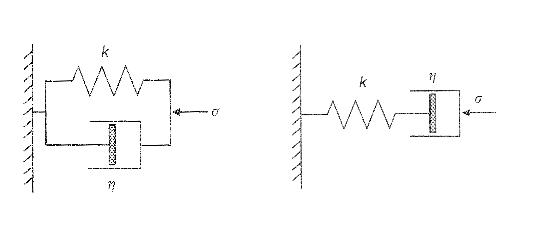
\includegraphics[width=0.95\textwidth]{figures/rheomod_vel.eps}
\caption{Mathematical modeling of reversible rate-dependent solid material behavior. Different combinations of a spring element with a
dashpot element \cite{JCZ:2007}: Kelvin-Voigt model (left) and Maxwell model (right)}
\label{fig:rheomod_vel}
\end{center}
\end{figure}

\newpage

The parallel connection of the spring and the dashpot elements is known as Kelvin-Voigt model. It is characterized by equal displacements
(and therefore equal strain values) in both of the individual elements, whereas the stress value of the model will be the sum of the
stresses in the spring and the dashpot. The constitutive behavior of the Kelvin-Voigt model is described by a differential equation.
\begin{equation}
\sigma\,=\,k\,\varepsilon\,+\,\eta\,\mathop{\varepsilon}\limits^{\miu{.}{}{}}
\label{eq:kelvin}
\end{equation}
If a stress $\sigma_0$ is instantaneously applied to a Kelvin-Voigt model, which is held constant thereafter, the solution of the
differential equation (\ref{eq:kelvin}) is given as follows:
\begin{equation}
\varepsilon\,=\,\frac{\sigma_0}{k}\,\left[1\,-\,\mathrm{e}^{-kt/\eta}\right]
\end{equation}
which indicates that the strain increases asymptotically to its steady-state (elastic) value $\sigma_0/k$. Thus, the Kelvin-Voigt model
represents the typical strain retardation, but neglecting any instantaneous strain.

The series connection of the spring and the dashpot elements is known as Maxwell model. Within this context, equal stress values occur in
both of the individual elements, whereas the total displacement (and therefore the strain) of the model will be the sum of the
displacements in the spring and the dashpot. The constitutive behavior of the Maxwell model can again be described by a differential
equation. 
\begin{equation}
\mathop{\varepsilon}\limits^{\miu{.}{}{}}\,=\,\frac{1}{\eta}\,\sigma\,+\,\frac{1}{k}\,\mathop{\sigma}\limits^{\miu{.}{}{}}
\label{eq:maxwell}
\end{equation}
Applying an instantaneous stress, a Maxwell element exhibits an instantaneous elastic response characterized by the spring constant $k$,
and a long-term viscous response specified by the viscosity $\eta$. If the Maxwell substance is subjected to an instantaneous jump in
strain with the amplitude $\varepsilon_0$, which is held constant thereafter, the differential equation (\ref{eq:maxwell}) can be solved closely.
The solution
\begin{equation}
\sigma\,=\,k\,\varepsilon_0\,\mathrm{e}^{-kt/\eta}
\end{equation}
indicates a stress decrease (relaxation) at constant (non-zero) strain, whereas in case of the Maxwell model the stress relaxes to zero,
simulating the behavior of a viscoelastic fluid.

\subsection{Viscoplasticity}
\label{sec:viscoplast}

Viscoplasticity is the most general material class, and the constitutive theories of viscoplasticity must be defined, on principle, to model all macroscopically observable phenomena of material behavior. The viscoplastic material class combines elements of all the other classes presented above. Micromechanical phenomena causing viscoplastic material behavior are exceptionally complex. 

Here, we will focus only on one typical effect of viscoplastic material behavior particularly relevant for geomaterials -- creep processes. Although in both cases characterizing the strain evolution at constant stress, viscoplastic creep differs from the viscoelastic creep (retardation) mentioned above, because no asymptotical strain value will be reached in the viscoplastic case. A typical viscoplastic creep curve is shown in Fig.~\ref{fig:creep}.

\begin{figure}[htb!]
\begin{center}
\footnotesize
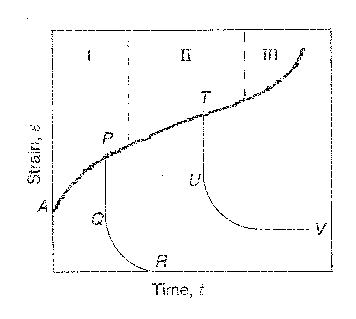
\includegraphics[width=0.5\textwidth]{figures/creep.eps}
\caption{Schematical representation of a viscoplastic creep curve showing the three typical periods: primary, secondary, and tertiary creep \cite{JCZ:2007}. The three periods are indicated by the Roman numerals I, II and III, the point $A$ indicates the instantaneous elastic strain}
\label{fig:creep}
\end{center}
\end{figure}

For the viscoplastic creep behavior, generally, three typical periods can be observed. Whereas at all creep periods strain increases without reaching any asymptotical value, they differ in the strain rate. The first period, called primary creep, is characterized by a decreasing creep rate (transient creep), while for the second creep period, called secondary creep, a constant strain rate is observed (stationary creep, steady-state creep). The period of more or less constant strain rate is followed by the tertiary creep with ever-inreasing strain rate, eventually causing mechanical failure of the structure under consideration. The total reduction of the applied stresses results in a strain relaxation. Unloading in the primary creep period is characterized by a complete strain relaxation (similar to viscoelatic behavior). However, if stress is removed during the secondary creep period, residual strains remain (effect of plasticity).

Comparable to theory of elastoplasticity, as starting point for the constitutive modeling of viscoplastic stress-strain states serves the functional relation between the stress rate and the elastic strain rate (\ref{eq:elplastmatlaw}). The overall strain tensor is additively decomposed into several constitutive parts: apart from the partial elastic and plastic strain tensors a creep strain tensor is introduced $\miu{\varepsilon}{\mathrm{c}}{}$.
\begin{equation}
\miu{\varepsilon}{}{\dot}\,=\,\miu{\varepsilon}{\mathrm{el}}{\dot}\,+\,\miu{\varepsilon}{\mathrm{pl}}{\dot}\,+\,\miu{\varepsilon}{\mathrm{c}}{\dot}
\label{eq:strainsplit_vpl}
\end{equation}
Similar to the plastic potential (yield condition), the creep behavior is mathematically characterized based on appropriately defined creep potentials $\Phi_{\mathrm{c}}(\miu{\sigma}{}{})$ representing, again, relationships among the coefficients of the stress tensor. Consequently, the creep strain rate tensor is defined as follows:
\begin{equation}
\miu{\varepsilon}{\mathrm{c}}{\dot}\,=\,
\lambda_{\mathrm{c}}\,\frac{\partial\Phi_{\mathrm{c}}(\miu{\sigma}{}{})}{\partial\miu{\sigma}{}{}}
\label{eq:creepstrainrate}
\end{equation}
with the so-called creep multiplier $\lambda_{\mathrm{c}}$. Consequently, the constitutive relation (\ref{eq:elplastmatlaw}) can be
reformulated. 
\begin{equation}
\miu{\sigma}{}{\dot}\,=\,\fourtens{C}
\left(\miu{\varepsilon}{}{\dot}\,-\,
\lambda_{\mathrm{pl}}\,\frac{\partial\Phi_{\mathrm{pl}}(\miu{\sigma}{}{})}{\partial\miu{\sigma}{}{}}
\,-\,
\lambda_{\mathrm{c}}\,\frac{\partial\Phi_{\mathrm{c}}(\miu{\sigma}{}{})}{\partial\miu{\sigma}{}{}}
\right)
\label{eq:vplastmatlawmod}
\end{equation}

In geomechanics, the long-term rock behavior during the stationary creep period is the main focus of interest. One widely-used creep potential characterizing secondary creep is the so-called Norton's model
\begin{equation}
\Phi_{\mathrm{c}}(\miu{\sigma}{}{})\,=\,
\frac{\alpha}{n+1}\,
\left(\sqrt{\ttfrac{3}{2}\miu{\sigma}{d}{}\ccdot\miu{\sigma}{d}{}}\right)^{n+1}
\label{eq:norton}
\end{equation}
with the material parameters $\alpha$ and $n$.

\vspace{4.0ex}
All of the constitutive models mentioned above are idealized approximations of the actual material behavior. The presented models are relatively simple, and allow to gain a first insight into the material theory of deformable solid substances. Some other aspects, which are relevant for rock mechanics analyzing material behavior could not be considered here, and are subject of further studies, like:
\begin{itemize}
\item Rate-dependent deformation processes in porous media are caused by the pore pressure diffusion through the solid skeleton at a finite rate, and intrinsic viscous properties of the matrix material. A separated experimental observation of theses effects is quite challenging with according consequences to the constitutive modeling.
\item Certain geomaterials show a layered structure (e.g. shale, sandstone). Consequently, material properties of these substances depend on the direction of the impact of external forces (known as anisotropic material behavior), which has to be considered in constitutive relations.
\item Damage and failure of rocks play an important role in real geoprocesses, and require an individual consideration.
\item The analysis of wave propagation (dynamic phenomena) in geomaterials is relevant for all kinds of seismic activities or seismic analyses.
\item The design of appropriate lab tests is essential for the fundamental characterization of the material behavior, and the calibration of constitutive models.
\end{itemize}

%-------------------------------------------------------------------------
\section{Porous medium properties}

We have considered the properties of fluid (section \ref{sec:fluid_properties}) and solid phases (section \ref{sec:m_properties}), respectively. Many of the properties of a porous medium can be determined based on the assumption of the local thermodynamic equillibrium allowing a superposition of phase related characteristics - except of the hydraulic properties for multiphase flow, which are discussed in this section in more detail. We restart with the different definitions of saturation.

\subsection{Saturation}

Saturation of a fluid phase $\gamma$ is defined as the volumetric fraction $\epsilon^\gamma$ related to the sum of all fluid phases volumetric fractions.
%
\begin{eqnarray}
S^\gamma =
\frac{\epsilon^\gamma}{\sum_{\gamma}\epsilon^\gamma}
\end{eqnarray}

The sum of saturations of all fluid phases must be equal to unity (section \ref{sec:mixtures}).
%
Effective saturation is defined as \cite{BroCor:64}
%
\begin{eqnarray}
S_{\mbox{\small eff}}^\gamma =
\frac{S^\gamma-S_r^\gamma}{1-S_r^\gamma}
\end{eqnarray}

Moisture content (volumetric water content) is defined as the
product of porosity and saturation.
\begin{eqnarray}
\theta^\gamma = n S^\gamma
\end{eqnarray}

Gravimetric water content is defined as
\begin{eqnarray}
\omega^\gamma
=
n S^\gamma
\frac{\rho_d^s}{\rho^\gamma}
\end{eqnarray}

Applying the chain rule, we can express saturation changes in
following way.
\begin{eqnarray}
dS^\gamma =
\frac{dS^\gamma}{dp^\gamma} dp^\gamma
\end{eqnarray}

The capillary pressure-saturation functions as well as the relations between relative permeability and saturation are substantial constitutive equations required for multiphase flow. Within this context, usually algebraic expressions are fit to the corresponding experimentally observed curves. Among the widely-used of these algebraic expressions are the Brooks-Corey \cite{BC:1964} and van Genuchten \cite{Van:80} relations. If both are realized within the scientific software code developed by the authors, the numerical results presented in this paper are based on Brooks-Corey's approach.

%---
\subsection{Capillary pressure and relative permeability}
\index{quantity - pressure capillary}

As a consequence of interfacial tension a discontinuity in fluid
pressure exists across the interface that separates two immiscible
fluids. The partial pressure difference between two phases is
denoted as capillary pressure, which is a function of saturation.
%
\begin{eqnarray}
p_c^{\alpha\beta} = p^\beta -
p^\alpha = f(S^\alpha)
\end{eqnarray}

In general, capillary pressure is the difference between partial
pressures of non-wetting and wetting phases.
\begin{eqnarray}
p_c = p^{nw} - p^w =
f(S^w) 
\label{eqn:capillary_pressure}
\end{eqnarray}

Capillary pressure is always positive: $p_c>0 ,
\forall S$. It is often assumed that air is at a constant
atmospheric pressure taken as zero $p^g=0$. This means,
the macroscopic pressure of water in the unsaturated zone is
always negative due to suction.
%
Capillary pressure must be measured for given soils and pairs of
fluids. In general, these experiments are conducted for
equilibrium conditions with no fluid in motion. Various authors
have proposed analytical functions for capillary pressure -
saturation - relationships. 

\begin{figure}[htb!]
\begin{center}
\includegraphics[width=0.43\columnwidth]{figures/HYSTER.EPS}
\caption{Capillary hysteresis \cite{Bea:72}, with
$S_{w} = S^w$, $S_{w0} =
S_r^w$, $S_{n} = S^{nw}$,
$S_{n0} = S_r^{nw}$ } 
\label{fig:hysteresis}
\end{center}
\end{figure}
%
\index{process - hysteresis capillary}

The capillary pressure/saturation relationships
differ for drainage and rewetting (imbibition) \cite{Mua:76}. This phenomenon is
called hysteresis (Fig. \ref{fig:hysteresis}). Reasons for capillary pressure hysteresis are:
(i) varying pore shape (ink-bottle effect), (ii) contact angle
hysteresis (raindrop effect), (iii) entrapment of non-wetting
fluids, (iv) swelling and shrinking of solid grains.

To introduce the concept of relative permeability we recall the
Darcy law for flow of multiple fluid phases through porous
media, equation (\ref{eqn:momentum_balance_fluid}).
Fig. \ref{fig:k_rel} shows an example of relative permeabilities for both wetting and non-wetting phases.

\begin{figure}[htb!]
\begin{center}
\includegraphics[width=0.45\columnwidth]{figures/K_REL.EPS}
\caption{Relative permeability functions \cite{Bea:72} with
$S_{w} = S^w$, $S_{w0} =
S_r^w$, $S_{n} = S^{nw}$,
$S_{n0} = S_r^{nw}$, $k_{rn} = k^{nw}$,
$k_{rw} = k^w$ } 
\label{fig:k_rel}
\end{center}
\end{figure}
%

We consider some of the most used models after van Genuchten, Haverkamp, Brooks-Corey.

%-------------------------------------------------------------------------------
\subsubsection*{van Genuchten model \cite{Van:80}}

The definitions of effective saturation, capillary pressure and relative permeability for the van Genuchten model are as follows
%
\begin{eqnarray}
S_{\mbox{\small eff}} = \frac{S^w - S_r^w}{1 -
S_r^w} = \left( 1 + (\alpha \, p_c)^n
\right)^m \qquad , \qquad p_c > 0
\end{eqnarray}
%
\begin{eqnarray}
p_c = \left\{
\begin{array}{ll}
0 & S^w >
S^w_{\mbox{\footnotesize max}}
\\
\frac{\rho^w g}{\alpha} (S_{\mbox{eff}}^{-1/m}-1)^{1/n} &
S_r^w < S^w <
S^w_{\mbox{\footnotesize max}}
\\
{p_c}_{\mbox{\footnotesize max}} & S^w <
S_r^w
\end{array}
\right.
\end{eqnarray}
%
with
\begin{eqnarray}
m = 1 - \frac{1}{n}
\end{eqnarray}
%
\begin{eqnarray}
\mathbf{k}_{\mbox{\small rel}}(h) 
= 
\frac{1-(\alpha h)^{n-2}\,[1+(\alpha h)^n]^{-m}}{[1+(\alpha h)^n]^{2m}}
\end{eqnarray}

Figs. \ref{fig:VanGenuhetenParameter} and \ref{fig:vG_krel} show the capillary pressure and relative permeability functions corresponding to the parameters given in Tab. \ref{tab:van_Genuchten}, respectively.

\begin{figure}[htb!]
\begin{center}
\includegraphics[width=0.7\columnwidth]{figures/VanGenuheten_P.eps}
\caption{Capillary pressure / saturation relationship (Tuebingen experiment
2005)} \label{fig:VanGenuhetenParameter}
\end{center}
\end{figure}
%

\begin{figure}[htb!]
\begin{center}
\includegraphics[width=0.6\columnwidth]{figures/VanGenuheten_K.eps}
\caption{Relative permeability / saturation relationship (Tuebingen experiment
2005)} 
\label{fig:vG_krel}
\end{center}
\end{figure}

% Tabelle als Gleitumgebung
\begin{table}[htb!]
\caption{Model parameter}
\label{tab:van_Genuchten}
\begin{center}
\begin{tabular}{|l|l|l|l|}
\hline
$S_r^w$     & residual water saturation &  $ 0 $   &   \\
$S^w_{max}$ & maximal water saturation   & $0.645$ & $$ \\
$n$         & vG parameter  & $4.8$ &  \\
$\alpha$    & vG coefficient  & $320$ & $[m^{-1}]$ \\
\hline
\end{tabular}
\end{center}
\end{table}
%

%-------------------------------------------------------------------------------
\subsubsection*{Haverkamp model \cite{HavVauTouWieVac:77}}

The formulas for the Haverkamp model are given in terms of pressure head
$h=p^w/g\rho^w$\index{quantity - pressure head}
and moisture content
$\theta=nS^w$.\index{quantity - moisture content}
%
The definitions of effective saturation, capillary pressure and relative permeability for the Haverkamp model are as follows
%
\begin{eqnarray}
\theta = \frac{\alpha(\theta_s-\theta_r)}{\alpha+|h|^\beta} +
\theta_r
\end{eqnarray}
\begin{eqnarray}
h = \left( -\frac{\alpha}{\theta} (\theta - \theta_s + \theta_r)
\right)^{1/\beta}
\end{eqnarray}
%
\begin{eqnarray}
\mathbf{k}_{\mbox{\small rel}}(h) = K_s \frac{A}{A+|h|^\beta}
\end{eqnarray}

%
% Tabelle als Gleitumgebung
\begin{table}[htb!]
\caption{Model parameter}
\label{tab:Haverkamp}
\begin{center}
\begin{tabular}{|l|l|l|l|}
\hline
$\theta$    & volumetric water (moisture) content &         & $[cm^3/cm^3]$ \\
$\theta_r$  & residual volumetric water content   & $0.075$ & $[cm^3/cm^3]$ \\
$\theta_s$  & saturated volumetric water content  & $0.287$ & $[cm^3/cm^3]$ \\
$h(\theta)$ & soil water pressure head            &         & $[cm]$ \\
            & relative to the atmosphere          &         & \\
$\alpha$    &                                     & $1.611\times 10^6$ & $[Pa^{-1}]$ \\
$\beta$     &                                     & $3.96$ & \\
\hline
\end{tabular}
\end{center}
\end{table}
%

Fig. \ref{fig:Haverkamp} shows the capillary pressure saturation function corresponding to the parameters given in Tab. \ref{tab:Haverkamp}.

% *** EPS-Grafik ***
\begin{figure}[htb!]
\begin{center}
\footnotesize
%\psfrag{Synonym}[pos][pos]{Tex-Ersetzung}
%\psfrag{x}[][]{$t$}
%\psfrag{y}[b][t]{$y(t)$}
%\psfrag{t}[][]{ }
\includegraphics[width=0.95\columnwidth]{figures/haver1.eps}
\caption{Hydraulic properties of unsaturated soil
\cite{HavVauTouWieVac:77}} 
\label{fig:Haverkamp}
\end{center}
\end{figure}
%

%-------------------------------------------------------------------------------
\subsubsection*{Brooks \& Corey model \cite{BroCor:64}}

The Brooks-Corey equations relating the saturation to the capillary pressure are
\begin{equation}
p^c\,=\,p^D\,S_{\mathrm{eff}}^{-(1/\lambda)}
\qquad\mbox{for}\qquad p^c\geq p^D
\label{eq29}
\end{equation}
%\begin{equation}
%S_{\mathrm{eff}}\,=\,
%\left\{
%\begin{array}{ccl}
%1                                                            & , & \quad p^c\leq p^D \\[2.0ex]
%\left(\frac{\textstyle{p^D}}{\textstyle{p^c}}\right)^\lambda & , & \quad p^c > p^D
%\end{array}
%\right.
%\label{eq29}
%\end{equation}
where $p^D$ is usually known as entry pressure, $\lambda$ is a pore-size distribution index.
%
$S_{\mathrm{eff}}$ is a normalized wetting fluid saturation. For the case of \co2 as wetting fluid into a saline aquifer it is defined as
\begin{equation}
S_{\mathrm{eff}}=\frac{S^{l}-S^l_{\mathrm{res}}}{1-S^l_{\mathrm{res}}-S^{CO_2}_{\mathrm{res}}} \\
\label{eq30}
\end{equation}
where $S^l_{\mathrm{res}}$ is the wetting phase residual or irreducible saturation, and $S^{CO_2}_{\mathrm{res}}$ is the nonwetting phase residual saturation. The constitutive parameters $p^D$, $\lambda$, $S^l_{\mathrm{res}}$ and $S^{CO_2}_{\mathrm{res}}$ are identified by fitting Eq.~(\ref{eq29}) to experimental data. Within this context, the entry pressure is to be understood as the minimum pressure that the nonwetting fluid must have to enter the largest pores. The relations between the relative permeability and the saturation are given by
\begin{eqnarray}
k_{\mathrm{rel}}^{l} & = & \left(S_{\mathrm{eff}}\right)^{(2+3\lambda)/\lambda}
\label{eq31} \\[2.0ex]
k_{\mathrm{rel}}^{CO_2} & = & \left(1-S_{\mathrm{eff}}\right)^2\,\left(1-\left(S_{\mathrm{eff}}\right)^{(2+\lambda)/\lambda}\right)
\label{eq32}
\end{eqnarray}



